\documentclass[11pt]{article}
\usepackage[margin=1in]{geometry}
\usepackage{amsmath,amssymb}
\usepackage{booktabs}
\usepackage{longtable}
\usepackage{graphicx}
\usepackage{hyperref}
\usepackage{natbib}

\title{Where Should Machine Learning Go in Hybrid Trading Systems?\\
Matched-Budget Component Attribution Across Three Markets}
\author{}
\date{Version 4 (refined, with open-source reference implementation) ---
\small code, data, and tests: \url{https://github.com/Cannonbold2412/ML_Component_Attribution}}

\begin{document}
\maketitle

\begin{figure*}[h]
  \centering
  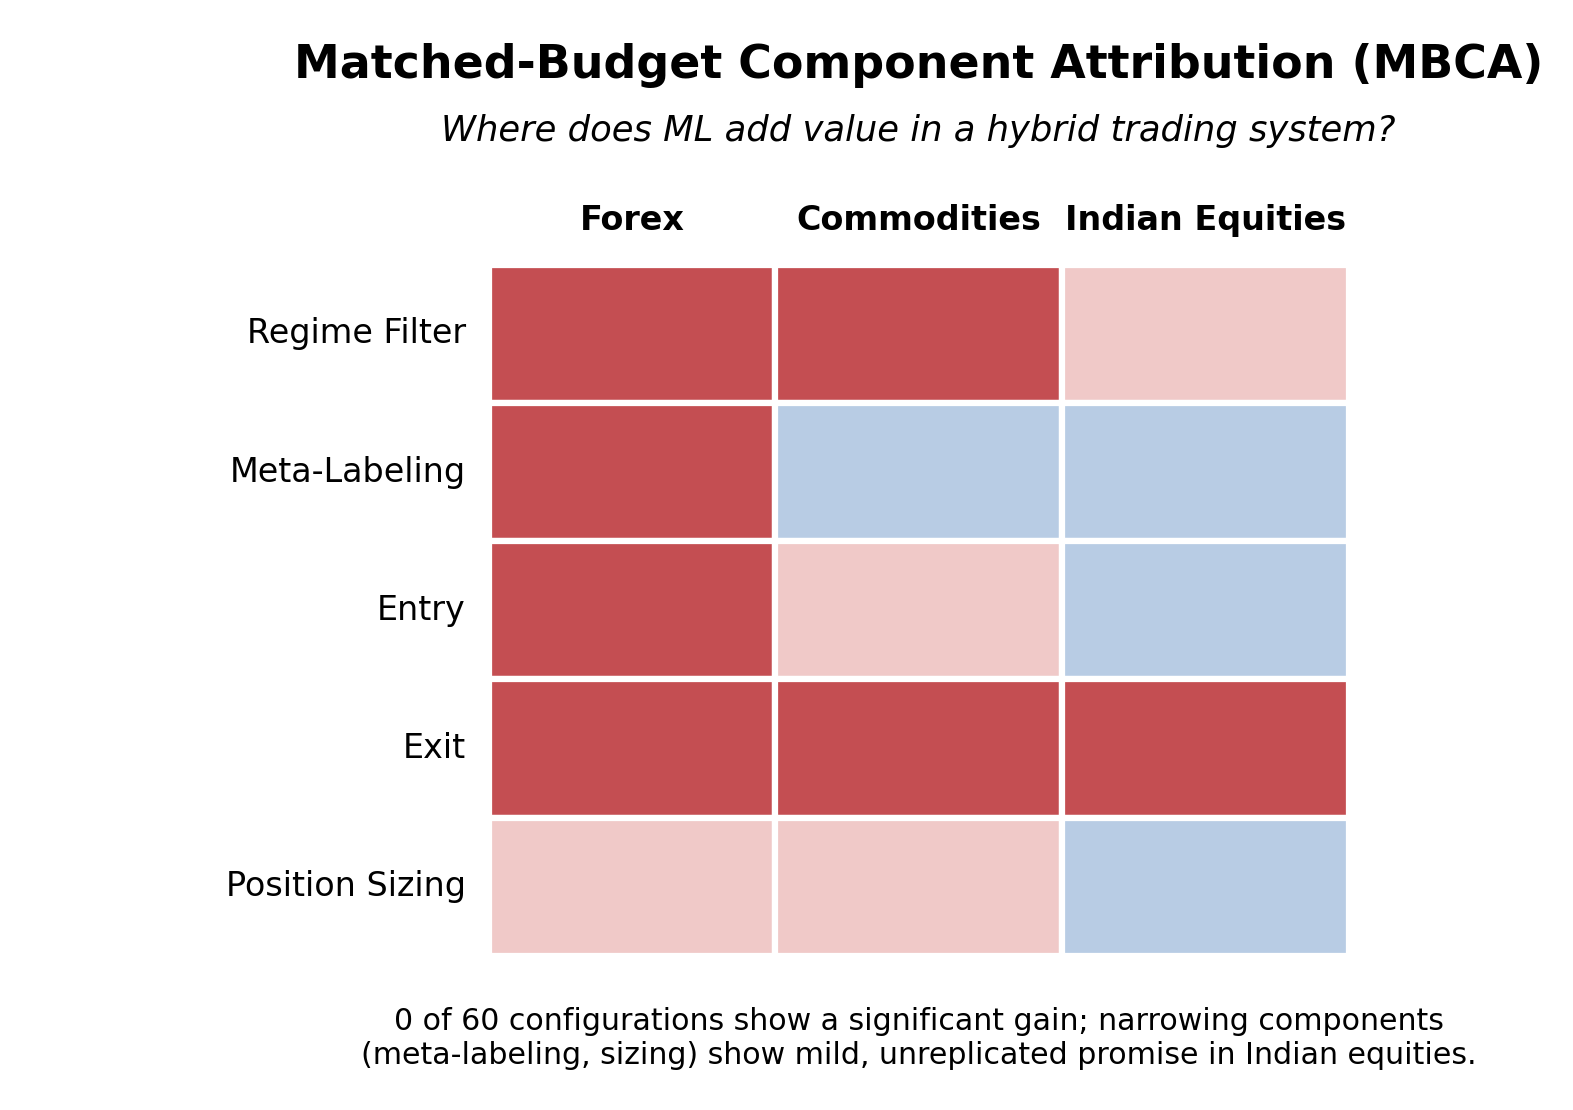
\includegraphics[width=0.55\textwidth]{figures/p36_graphical_abstract.png}
\end{figure*}

\begin{abstract}
Hybrid trading systems that combine rule-based signal generation with machine-learned components
are common in practice, but the literature rarely asks a decomposable question: at which specific
decision point does an ML component actually help, and where does it hurt? We introduce
\textbf{Matched-Budget Component Attribution (MBCA)}, a general-purpose methodology for answering
that question in any hybrid decision system: hold a validated rule-based control fixed, replace
exactly one insertion point at a time with a matched-budget machine-learned counterpart ---
identical features, identical model class, identical evaluation protocol --- and report every
resulting configuration's forward-tested statistical significance, not only the configuration that
happened to look best. We apply MBCA to one already-validated rule-based trading strategy --- a JMA
fast/slow crossover with an ATR stop/target (or trailing) exit stack, validated with a strict freeze
$\to$ holdout $\to$ forward-tail protocol on three markets (forex, commodities, Indian equities) ---
across five insertion points that span a natural component taxonomy: an \emph{independent}
bar-level gate (regime filter); two \emph{narrowing} components that filter or re-weight decisions
the rule-based system already makes (meta-labeling, position sizing); and two \emph{replacing}
components that substitute the rule-based mechanism outright (entry generation, exit policy). Every
component shares the same 8 backward-only features, the same LightGBM configuration, the same
freeze discipline, and the same deflated-Sharpe / bootstrap-CI statistical stack.

Across 5 individual components plus 4 combination experiments (Entry+Exit, Entry+Sizing,
Exit+Sizing, and an empirically-chosen Best Combined pairing of Meta-Labeling with Position Sizing)
$\times$ 3 markets $\times$ 2 evaluation windows --- 60 testable configurations with a bootstrap CI
available --- \textbf{zero show a statistically significant improvement over the rule-based
baseline}, while 20 show a statistically significant loss. We summarize the full grid as the
\textbf{ML Opportunity Matrix}, a component/combination $\times$ market decision-support artifact
with a mechanically-derived recommendation column, and a companion decision flowchart. The evidence
is component-specific and market-specific, not uniform: narrowing components are gentler and
occasionally directionally positive, concentrated in Indian equities, while replacing components
are more volatile and, for exit specifically, actively harmful --- ML Exit inflates trade count
2.7$\times$--4.2$\times$ (early learned exits un-block JMA crossovers a longer-held rule-based trade
would have absorbed) and loses significantly in 4 of 5 tested configurations. On the original forex data,
every ML intervention tried loses (a finding the independent replication does not reproduce). Best Combined --- Meta-Labeling filtering trades, then Position Sizing
re-weighting the survivors --- produces the campaign's single closest-to-significant result:
Indian-equities holdout Sharpe 2.84 $\to$ 4.01 (bootstrap CI on the per-day Sharpe difference
$[-0.050, 0.176]$, i.e.\ roughly $[-0.8, 2.8]$ in annualized units) and forward Sharpe
1.05 $\to$ 2.70 (CI $[-0.087, 0.293]$, roughly $[-1.4, 4.7]$ annualized), with a directionally consistent, non-significant improvement
in commodities on both windows too. The paper's contribution is MBCA itself, the ML Opportunity
Matrix and decision framework it produces, and the resulting map of where ML helps, hurts, or is a
wash in one concrete hybrid system --- not a claim of a validated ML-enhanced trading strategy,
which the evidence here does not support, though Best Combined in Indian equities is the one
configuration worth a second-freeze-date replication before ruling out entirely. An independent,
open-source re-implementation of the full protocol (\texttt{mbca}, released with this paper)
reproduces the headline --- 0 of 60 significant improvements, ML Exit significantly harmful in every
market via the same turnover mechanism, 49 of 60 configurations agreeing in sign --- but not the
paper's forex result, and only half of Best Combined's near-miss (see the Independent Replication
section).
\end{abstract}

\noindent\textbf{Keywords:} matched-budget component attribution, hybrid decision systems,
component taxonomy, ML opportunity matrix, decision framework, meta-labeling, regime filtering,
walk-forward validation, deflated Sharpe ratio, JMA, ATR

\section{Introduction}

A large fraction of practitioner and academic ``ML for trading'' work reports one hybrid
configuration --- a rule-based signal gated, filtered, or replaced by a learned model --- against
a baseline, and treats a Sharpe improvement (or lack of one) as evidence about ``machine learning
in trading'' generally. This conflates two very different questions: \emph{does ML help}, and
\emph{does ML help at THIS specific decision point, with THIS feature set and model class, holding
everything else fixed}. A hybrid pipeline has several natural insertion points --- which bars are
admissible (regime filter), whether a specific signal-fired trade should be taken (meta-labeling),
which bars generate entries at all (entry generation), when to exit (exit policy), and how much
capital to risk per trade (position sizing) --- and a single aggregate comparison cannot say which
of these, if any, is where the reported improvement (or degradation) actually comes from.

We introduce \textbf{Matched-Budget Component Attribution (MBCA)} to answer that decomposed
question directly and reproducibly. MBCA is a controlled-variable methodology for any hybrid
decision system that combines a rule-based control with learned components: hold the data, the
feature set, the model class and hyperparameters, the training/freeze discipline, and the
evaluation protocol fixed, and vary only \emph{which single insertion point} the ML component
replaces. Because every comparison shares an identical budget, a resulting Sharpe delta can be
attributed to the insertion point itself rather than to a confound of feature-engineering effort,
tuning effort, or dataset choice that would otherwise differ from one paper's hybrid configuration
to the next.

This paper demonstrates MBCA on one already-validated rule-based system: a JMA fast/slow crossover
with an ATR-based stop/target (or trailing-stop) exit, tested with a strict freeze $\to$ holdout
$\to$ forward-tail protocol on three markets (a 4-pair forex sleeve, a 5-instrument commodities
sleeve, and a 48-stock Indian-equities sleeve with annual sector curation) that this research
program had already validated as a standalone rule-based strategy before any ML was introduced. We
hold the dataset, features, model class (LightGBM, identical hyperparameters), training procedure,
freeze discipline, transaction costs, and evaluation protocol fixed, and replace exactly one
component at a time with its ML counterpart.

\textbf{Research question:} \emph{Where, specifically, does replacing one component of an
already-validated hybrid decision system with a matched-budget machine-learned counterpart create
value --- and where does it instead destroy value or do nothing?}

Applying MBCA to this system surfaces a taxonomy of insertion points by how much they can alter the
rule-based system's decisions: \emph{independent} components (a bar-level gate orthogonal to the
entry signal), \emph{narrowing} components (filter or re-weight decisions the rule-based system
already makes), and \emph{replacing} components (substitute the rule-based mechanism outright).
Across 60 tested configurations, narrowing components show a mild, non-significant,
market-concentrated positive pattern; replacing components perform worse, sometimes
catastrophically; and the independent regime filter is a dead end everywhere tested. We package
this evidence as the \textbf{ML Opportunity Matrix} (Figure~\ref{fig:matrix}), a compact
decision-support artifact, and a companion decision flowchart (Figure~\ref{fig:decision}).

\textbf{Contributions.}
\begin{itemize}
  \item \textbf{MBCA}, a matched-budget, controlled-variable methodology for attributing ML's
        contribution to a specific insertion point in a hybrid decision system, reusable beyond
        this trading strategy and, we argue, beyond trading (Section~\ref{sec:discussion}).
  \item A \textbf{component taxonomy} (independent / narrowing / replacing) that predicts, ex ante,
        which insertion points are gentler or more volatile to convert to ML.
  \item The \textbf{ML Opportunity Matrix} and an accompanying \textbf{decision flowchart} ---
        reusable artifacts that turn a 60-row results table into a practical, mechanically-derived
        recommendation per component per market.
  \item A full evidence grid across 5 components, 4 combinations, 3 markets, and 2 evaluation
        windows (60 configurations, none cherry-picked), including the losses.
\end{itemize}

\section{Research Gap}

Ablation studies of ML-augmented trading pipelines exist (e.g.\ a 2025 cross-sectional A-share
turnover pipeline ablates its component modules and attributes annualized-return contribution per
module; see Section~\ref{sec:related}), but they typically ablate \emph{modules of one specific
proprietary pipeline architecture}, not \emph{insertion points of a single control mechanism into
an already-fixed rule-based strategy} with identical features/model/hyperparameters held across
every component. No work we found formalizes this constraint as a named, reusable methodology, runs
the same feature set and model class through five distinct insertion points of one rule-based
strategy with a uniform freeze/holdout/forward-tail protocol and bootstrap-CI significance testing
at every insertion point, and reports the full grid of results --- including the (numerous) negative
ones --- as a decision-support artifact rather than the single configuration that happened to look
best. MBCA fills that gap: it is the methodology, not merely the experiment, that is missing from
the literature.

\section{Related Work}
\label{sec:related}

\textbf{Meta-labeling.} L\'opez de Prado's meta-labeling \citep{lopezdeprado2018afml} separates the
``which direction'' decision (the primary model) from ``should I take this specific signal'' (a
secondary classifier trained on realized outcomes) --- exactly the mechanism this paper's ML
Meta-Labeling component implements, though the primary model here is a fixed rule (JMA crossover),
not a learned one. In MBCA's taxonomy (Section~\ref{sec:taxonomy}), meta-labeling is a canonical
\emph{narrowing} component: it can only reject decisions the primary system already made, never
invent new ones.

\textbf{Regime-conditioned and hybrid rule+ML systems.} A 2026 hybrid system integrating technical
rules, ML, and financial sentiment for regime-adaptive equity strategies
\citep{generatingalpha2026hybrid} reports aggregate improvements over a rule-only baseline but does
not decompose which sub-component is responsible --- precisely the conflation MBCA is designed to
resolve. A 2025 deep-learning-enhanced, multi-day-turnover A-share pipeline
\citep{turnover2025ablation} is the closest methodological precedent we found: it ablates its five
pipeline modules one at a time and reports each module's marginal contribution to annualized return
--- the same spirit as MBCA's attribution table, but over a different, proprietary module set,
without a uniform ML feature/model budget held across modules, without a named, reusable
methodology, and without holdout-to-forward-tail generalization testing per module.

\textbf{Position sizing and volatility-managed portfolios.} Moreira and Muir's volatility-managed
portfolios \citep{moreira2017volmanaged} scale exposure by a \emph{realized-volatility} signal at
the portfolio level; this paper's ML Position Sizing component instead scales exposure by a
\emph{predicted-win-probability} signal at the individual-trade level --- another \emph{narrowing}
component in MBCA's taxonomy, since it re-weights rather than rejects.

\textbf{Time-series momentum.} Moskowitz, Ooi and Pedersen \citep{moskowitz2012momentum} is the
standard reference for the rule-based trend-following family this paper's baseline belongs to; our
contribution is orthogonal to theirs.

\textbf{Gap.} No work we found holds a rule-based strategy, its data, its features, its model
class, and its evaluation protocol fixed while sweeping which single component ML replaces, names
and formalizes that constraint as a reusable methodology, and reports every resulting
configuration's forward-tested significance rather than the best one. MBCA is that methodology;
this paper is its first full application.

\section{Methodology}
\label{sec:methodology}

\subsection{Matched-Budget Component Attribution (MBCA)}
\label{sec:mbca}

\textbf{Definition.} MBCA is a controlled-variable methodology for decomposing a hybrid decision
system's performance by insertion point. It applies whenever a system combines a validated,
rule-based control with one or more points where a learned model could instead make the decision.
MBCA holds five things fixed across every tested insertion point:
\begin{itemize}
  \item the \textbf{data} each component's model is trained and evaluated on;
  \item the \textbf{feature set} available to every learned component;
  \item the \textbf{model class and hyperparameters} (no per-component tuning);
  \item the \textbf{training/freeze discipline} (fit once, never refit on evaluation data); and
  \item the \textbf{evaluation protocol and statistical test} used to call a result significant.
\end{itemize}
Only the \emph{insertion point} --- which single decision in the pipeline the learned model
replaces or modifies --- is allowed to vary between configurations. This is what makes the
resulting Sharpe deltas attributable to the insertion point itself, rather than to a confound of
feature-engineering effort, tuning budget, or evaluation leniency that differs across papers
reporting different hybrid configurations. A negative result under MBCA is a statement about
\emph{this specific, stated budget} at that insertion point, not a universal claim that no learned
model could ever help there (Section~\ref{sec:limitations} returns to this point).

\subsection{A taxonomy of insertion points}
\label{sec:taxonomy}

Not every insertion point is equally exposed to failure. We classify each tested component by how
much it can alter the trade set the rule-based system would otherwise produce:

\begin{itemize}
  \item \textbf{Independent} --- gates admissibility orthogonally to the entry signal; can only
        reject bars, never alter the signal itself. \emph{Tested here:} Regime Filter.
  \item \textbf{Narrowing} --- filters or re-weights a decision the rule-based system already made;
        cannot invent trades the rule-based system would not have taken. \emph{Tested here:}
        Meta-Labeling, Position Sizing.
  \item \textbf{Replacing} --- substitutes the rule-based mechanism outright; can generate a
        materially different trade set. \emph{Tested here:} Entry, Exit.
\end{itemize}

We hypothesize, ex ante, that narrowing components bound their own worst-case damage (they can only
subtract or re-weight, never add spurious decisions) and should therefore show gentler,
lower-variance effects than replacing components, which can generate an entirely different trade
set and therefore carry more variance in both directions. Section~\ref{sec:results} tests this
hypothesis directly; Figure~\ref{fig:pipeline} shows where each category sits in the pipeline.

\begin{figure*}[h]
  \centering
  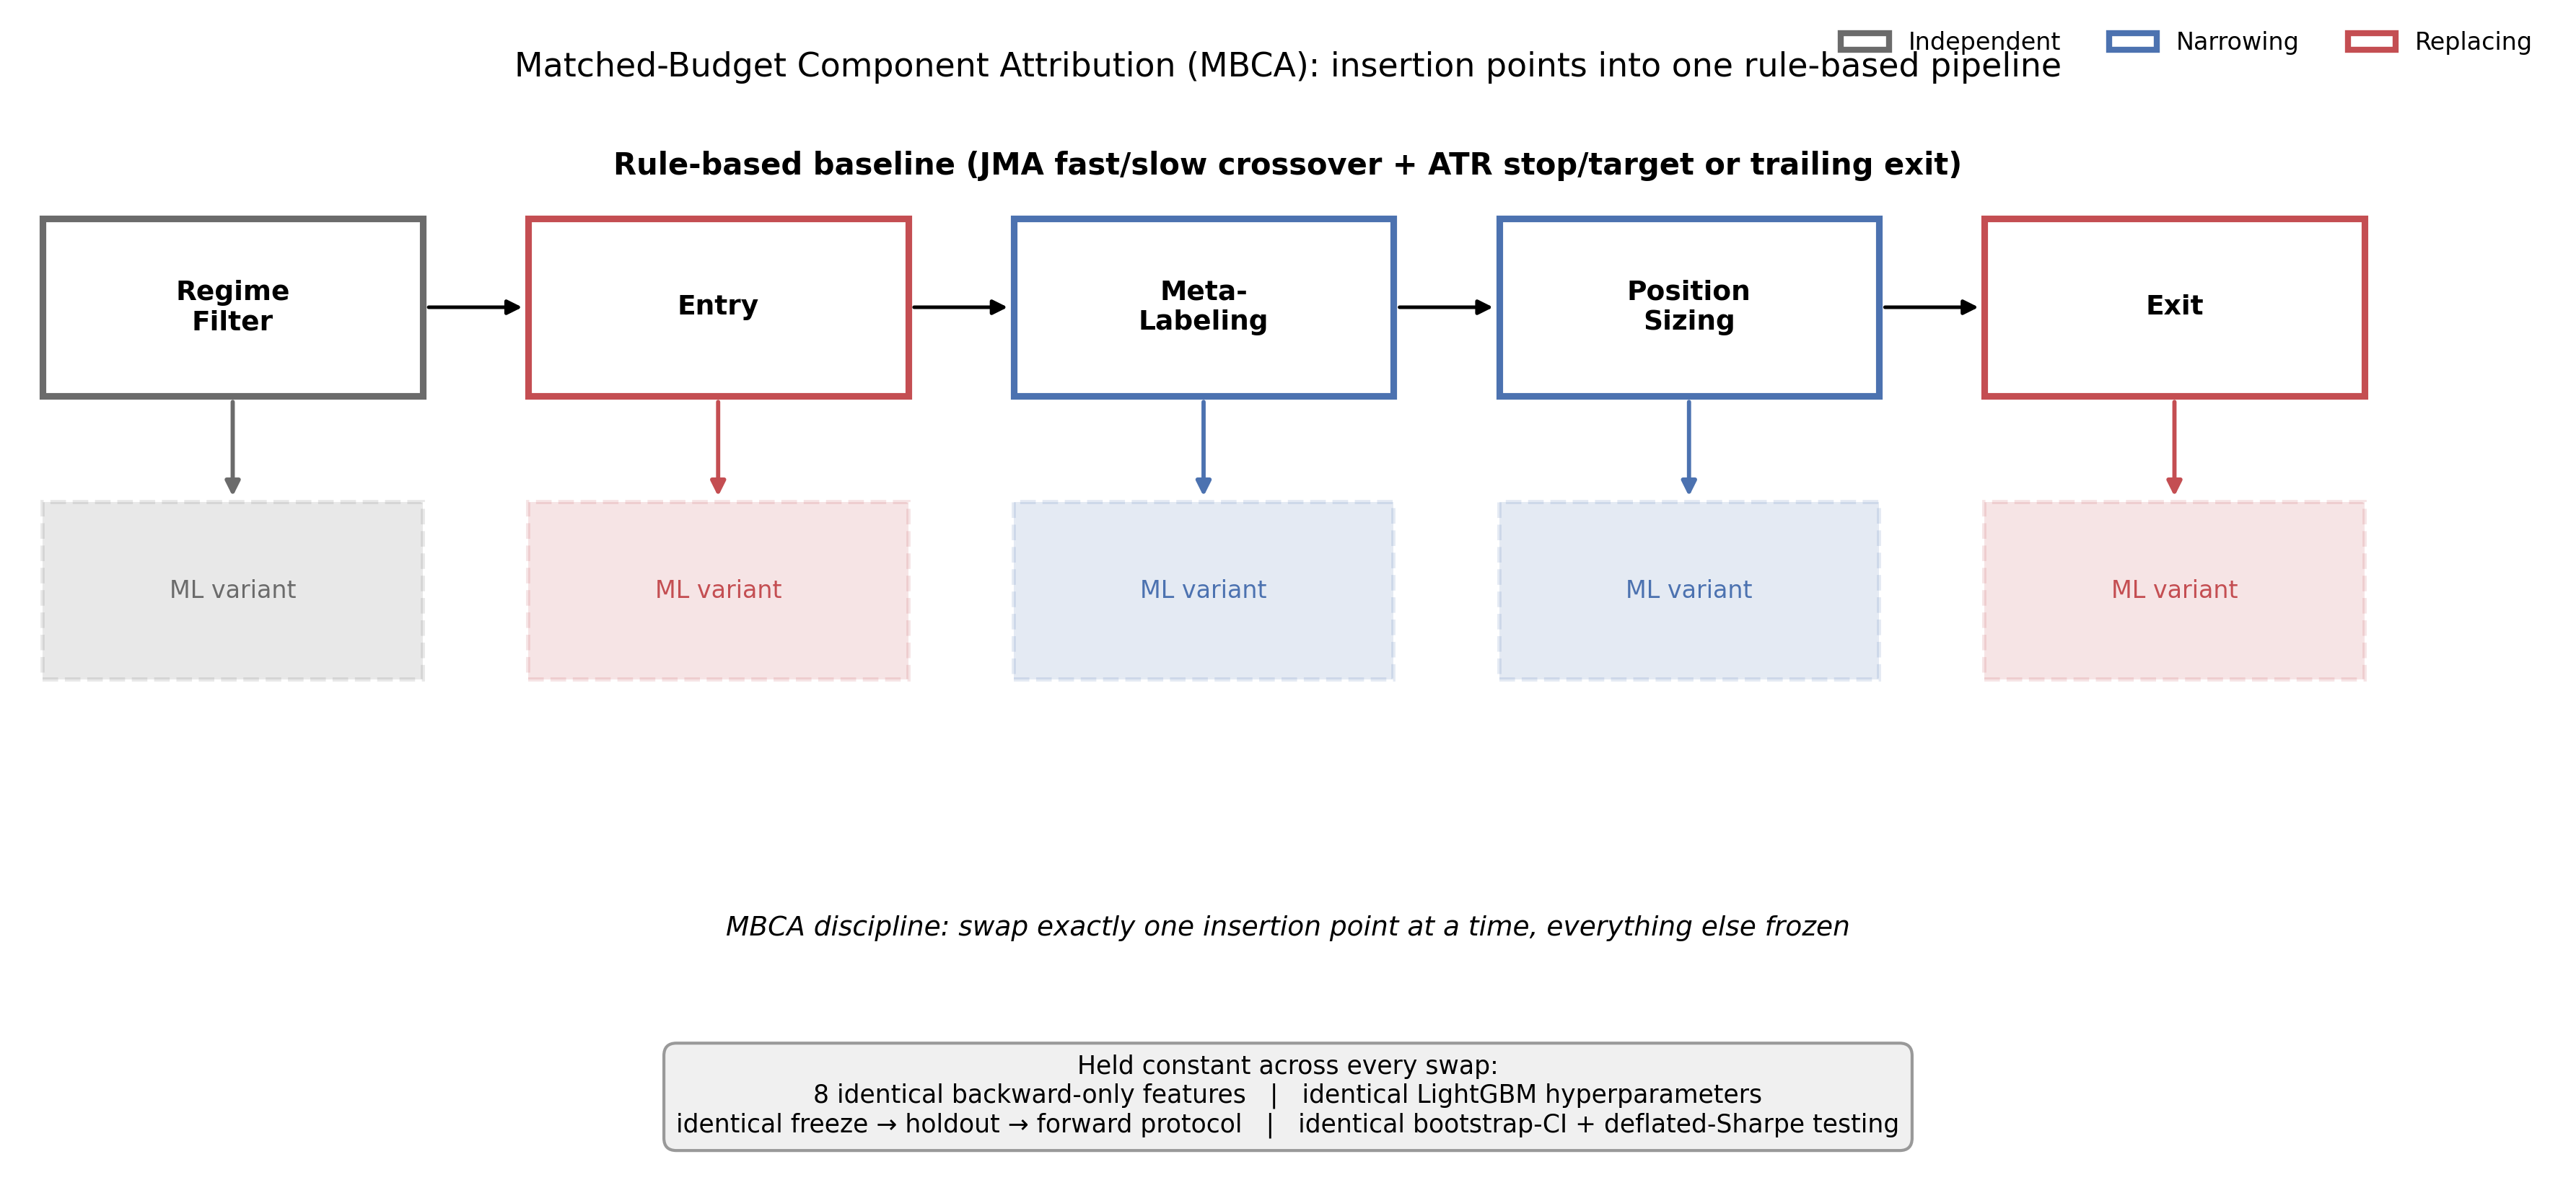
\includegraphics[width=\textwidth]{figures/p36_fig_mbca_pipeline.png}
  \caption{The MBCA experiment: five insertion points into one rule-based pipeline, each with a
  matched-budget ML counterpart, and the invariants held constant across every swap.}
  \label{fig:pipeline}
\end{figure*}

\subsection{The rule-based baseline (the MBCA control)}

A JMA(7)/JMA(21) fast/slow crossover generates entries; exits are either a fixed 1.5$\times$ATR
stop / 3$\times$ATR target bracket (forex) or a 1.5$\times$ATR stop with a 2$\times$ATR ratcheting
trailing stop (commodities and Indian equities) --- the exit mechanism each market's own prior
validation history in this repository selected before any ML work began. Position sizing is
uniform (fixed-fractional risk). This baseline is our control: it is re-run inside every
component's own campaign script, so every comparison in this paper is against a freshly regenerated
baseline under that exact campaign's conditions.

\subsection{Markets and data}

\begin{itemize}
  \item \textbf{Forex (4-pair):} AUDNZD, CADJPY, AUDUSD, NZDUSD, daily, already spans to present
        (no separate forward tail).
  \item \textbf{Commodities:} WTI, NATGAS, Brent, Gold, Silver, daily, with a separately-fetched
        forward tree.
  \item \textbf{Indian equities:} 48 NIFTY-50 constituents, daily, with annual rolling sector
        curation applied identically to every variant's trade book, and a separately-fetched
        forward tree.
\end{itemize}

Crypto was not included in this campaign: daily crypto data exists in this repository but has no
equivalent pre-ML validated baseline or forward-tail tree yet. We report this as a scope
limitation, not a null result.

\subsection{Components tested}

Rule-based baseline; ML Regime Filter (\emph{independent}; LightGBM trend/chop classifier gates
entries, 3 label definitions); ML Meta-Labeling (\emph{narrowing}; LightGBM classifier filters
signal-fired trades by predicted P(win)); ML Entry (\emph{replacing}; two LightGBM classifiers
generate entries directly, replacing \texttt{jma\_signals}); ML Exit (\emph{replacing}; two
LightGBM classifiers decide hold/exit per bar, replacing the ATR exit stack); ML Position Sizing
(\emph{narrowing}; the same frozen model as Meta-Labeling, consumed as a continuous capital
multiplier instead of a threshold); and four combinations (Entry+Exit, Entry+Sizing, Exit+Sizing,
Best Combined), detailed in Section~\ref{sec:combinations}.

Meta-Labeling and Position Sizing deliberately share one frozen model --- identical features,
label, and hyperparameters --- differing only in whether its output is thresholded (accept/reject)
or used as a continuous multiplier, isolating ``threshold vs.\ scale'' as the single manipulated
variable between those two narrowing components.

\subsection{Shared feature set and model}

All components use the identical 8 backward-only features: ADX, ATR-normalized momentum,
historical volatility, return z-score, backward-looking $R^2$, RSI, MACD histogram, and KAMA
slope --- every one computable from data up to and including bar $t$, none from future bars. Every
classifier is a \texttt{lightgbm.LGBMClassifier} with identical hyperparameters
(\texttt{n\_estimators=200, num\_leaves=31, max\_depth=6, learning\_rate=0.05,
min\_child\_samples=30, class\_weight="balanced"}, fixed \texttt{random\_state=42}) --- no
hyperparameter sweep for any ML component. This uniformity is the core MBCA constraint
(Section~\ref{sec:mbca}): sweeping hyperparameters per component would confound component
differences with tuning-effort differences, undermining the very attribution this paper sets out to
make.

\subsection{Freeze discipline}

Every classifier is fit exactly once, on a pre-split slice of each market's own data (a
70\%-of-calendar-span split). Training rows whose label lookahead window would cross the split date
are excluded --- enforced and unit-tested per component. After freezing, a classifier only ever
predicts; none of the components refit on holdout or forward data. Enforced freeze discipline is
essential to MBCA's validity: any refit on evaluation data would confound result interpretation
with dataset-selection bias.

\subsection{Evaluation windows and statistics}

Two windows per market where available: \textbf{holdout} (same processed tree the classifier
trained on, \texttt{entry\_time} $\geq$ split date) and \textbf{forward} (a genuinely
separately-fetched tree the classifier never saw during training or holdout evaluation). Forex has
no forward tree, reported as a limitation. Every comparison reports trade count, Sharpe ratio,
max drawdown, deflated Sharpe ratio (\texttt{n\_trials} set to the actual number of variants
screened within that component), and a 95\% bootstrap confidence interval of the difference in
Sharpe between the ML variant and that same campaign's own baseline. A result is significant iff
this CI excludes zero.

\textbf{Conventions, stated precisely.} (i) A trade stream is converted to a daily return series
by averaging the returns of all trades that \emph{exit} on each date (realized-at-exit, not
mark-to-market). (ii) Reported Sharpe ratios are annualized ($\sqrt{252}$) excess-return Sharpe
ratios with a 6\%/yr risk-free rate and population standard deviation. (iii) The bootstrap draws
2{,}000 replicates, resampling each variant's daily series \emph{independently} with replacement
(i.i.d., unpaired, fixed seed), and computes the difference of \emph{per-day, non-annualized}
Sharpe ratios (mean/std); CI bounds are therefore on a scale $\sqrt{252}\approx 15.9$ times smaller
than the annualized $\Delta$Sharpe reported beside them. Earlier drafts described this test as a
paired, instrument-level block bootstrap; that description was incorrect (see
Appendix~\ref{sec:errata}). Because the ML variant and its baseline trade the same instruments
over the same days, their daily returns are typically positively correlated, and ignoring that
pairing widens the interval (conservative); conversely, i.i.d.\ resampling ignores serial
dependence, which can narrow it. The reference implementation exposes both the paper's test and a
date-paired alternative (\texttt{run\_mbca(..., paired\_ci=True)}).

\section{Mathematical Formulation}

For bar $t$ in instrument $i$, $\mathbf{x}_{i,t} \in \mathbb{R}^8$ is the backward-only feature
vector defined above, identical across all five components.

\textbf{ML Regime Filter:}
$\hat{y}^{\text{regime}}_{i,t} = \mathbb{1}[P(\text{trend}_{i,t}=1\mid\mathbf{x}_{i,t}) \geq 0.5]$,
where $\text{trend}_{i,t}$ is one of three self-labeled forward-window definitions.

\textbf{ML Meta-Labeling:} at each bar where the primary rule fires
($\text{signal}_{i,t}\neq 0$), let $r_{i,t}$ be the realized return of the trade the primary rule
would open. The label is $y^{\text{meta}}_{i,t} = \mathbb{1}[r_{i,t}>0]$;
$\hat{p}^{\text{meta}}_{i,t} = P(y^{\text{meta}}_{i,t}=1\mid\mathbf{x}_{i,t})$ is estimated only at
signal-fired bars, and the trade is taken iff $\hat{p}^{\text{meta}}_{i,t}\geq 0.5$.

\textbf{ML Entry:} two classifiers estimate, for direction $d\in\{+1,-1\}$, whether a hypothetical
bracket entered at bar $t$ (stop $= \text{close}_t - d\cdot 1.5\cdot\text{ATR}_t$, target $=
\text{close}_t + d\cdot 3.0\cdot\text{ATR}_t$) hits target before stop within a 40-bar horizon:
$\hat{p}^{\text{entry}}_{d,i,t} = P(\text{target-first}\mid\mathbf{x}_{i,t}, d)$. The realized
signal is $\text{sign}(\arg\max_d \hat{p}^{\text{entry}}_{d,i,t})$ where that maximal probability
also clears 0.5, else flat.

\textbf{ML Exit:} two classifiers estimate, for a position already open in direction $d$, whether
price will still be favorable 10 bars ahead:
$\hat{p}^{\text{exit}}_{d,i,t} = P(d\cdot(\text{close}_{t+10}-\text{close}_t)>0\mid\mathbf{x}_{i,t})$,
evaluated at every bar while the position is open. Exit fires at the first bar
$\hat{p}^{\text{exit}}_{d,i,t}<0.5$, or at a 3$\times$ATR safety-net stop, whichever comes first.

\textbf{ML Position Sizing:} reuses $\hat{p}^{\text{meta}}_{i,t}$, consumed as a continuous
multiplier: $m_{i,t} = \text{clip}(2\cdot\hat{p}^{\text{meta}}_{i,t}, 0, 2)$, and every trade's
realized return is scaled: $r'_{i,t} = m_{i,t}\cdot r_{i,t}$.

\textbf{Generalization gap and significance:} for metric $M$ and component $c$,
$\Delta M_c = M_{\text{ML}}(c) - M_{\text{baseline}}$, per market and window. Significance is
assessed by an unpaired i.i.d.\ bootstrap of the two daily return series (2{,}000 replicates):
with $\widehat{SR}(r)=\bar r/s(r)$ the per-day Sharpe ratio and $r^{*}$ a resample, the 95\% CI is
the 2.5th/97.5th percentile of $\widehat{SR}(r^{*}_{\text{ML}})-\widehat{SR}(r^{*}_{\text{base}})$
across replicates; a result is called significant iff the CI excludes zero.

\section{Results: Component Attribution}
\label{sec:results}

Table~\ref{tab:attribution} reports every component $\times$ market $\times$ window combination
with a bootstrap CI available (40 rows, individual components only; combinations follow in
Section~\ref{sec:combinations}). \textbf{0 of 40} configurations show a significant improvement;
\textbf{10 of 40} show a significant loss. Figure~\ref{fig:matrix} summarizes the same evidence,
plus the four combinations, as the ML Opportunity Matrix; Figure~\ref{fig:attribution_forest} shows
the full per-configuration forest plot.

\begin{figure*}[h]
  \centering
  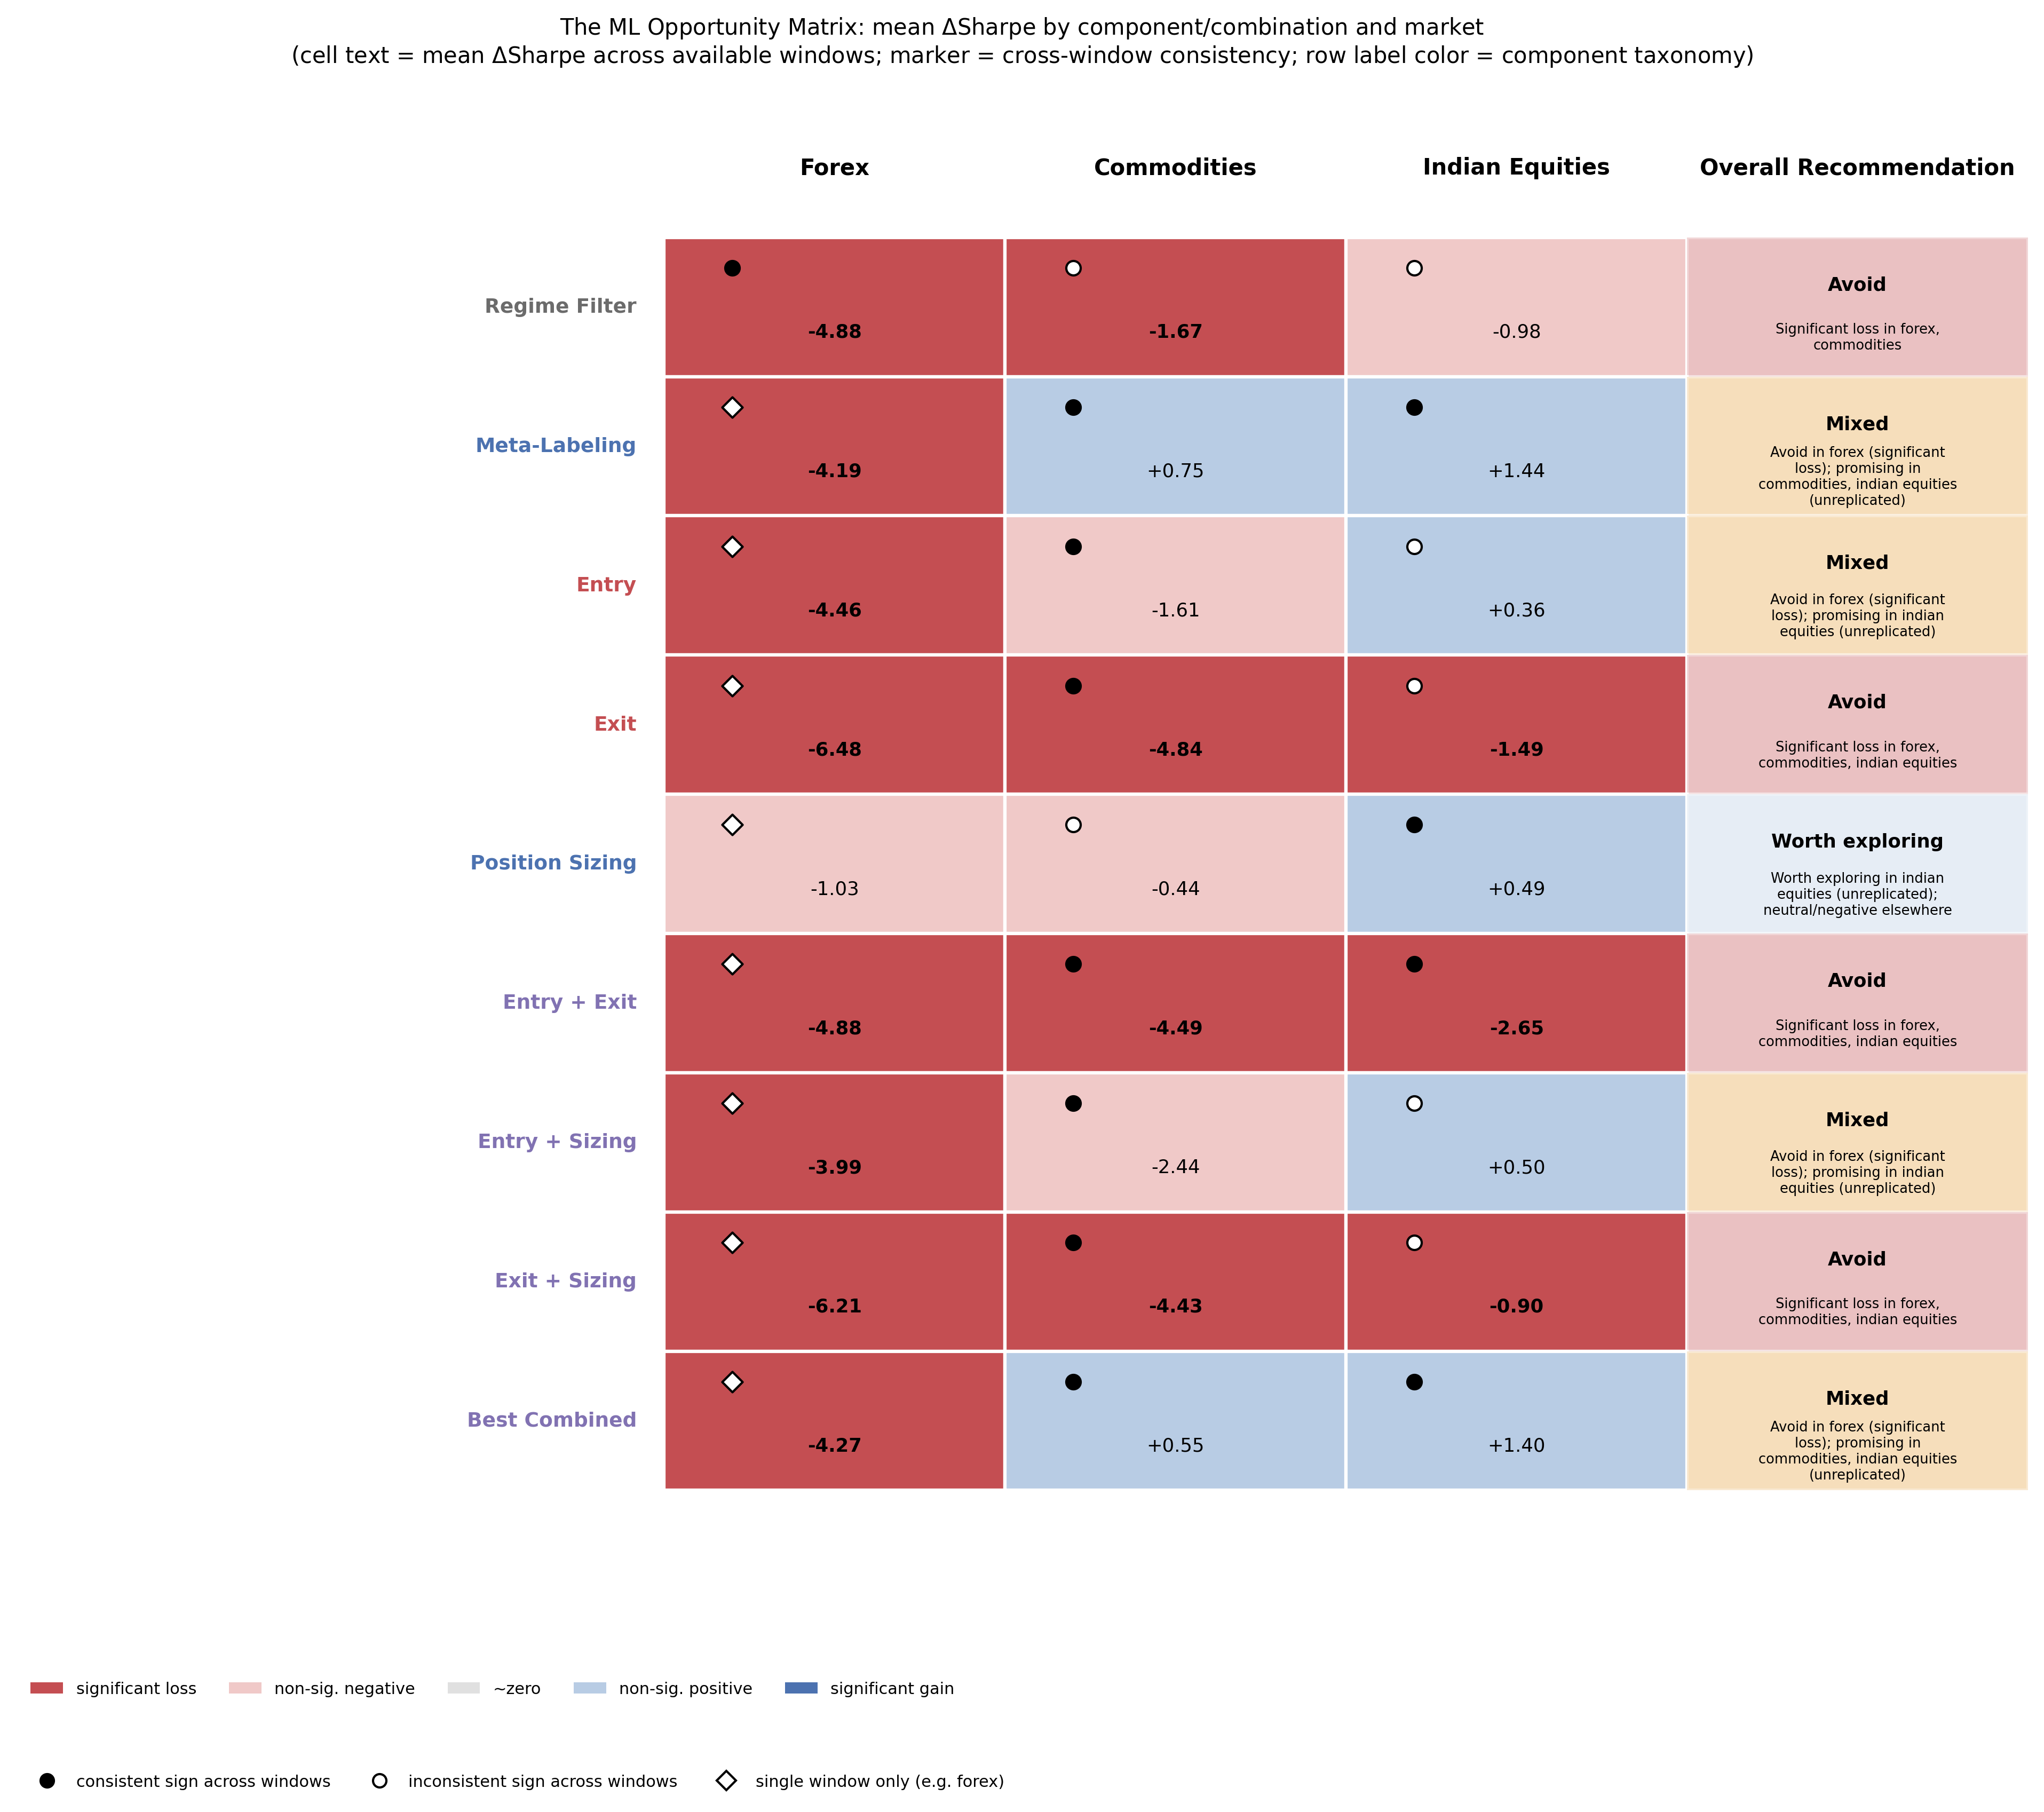
\includegraphics[width=\textwidth]{figures/p36_fig_opportunity_matrix.png}
  \caption{The ML Opportunity Matrix (flagship): every component and combination against every
  market, with a mechanically-derived Overall Recommendation. Cell color encodes effect direction
  and significance; marker encodes cross-window consistency; row-label color encodes the taxonomy
  of Section~\ref{sec:taxonomy}. Recommendations follow directly from significance, sign, and
  consistency (Section~\ref{sec:mbca}); none are hand-picked.}
  \label{fig:matrix}
\end{figure*}

\begin{longtable}{p{2.6cm} p{3.3cm} l l r r l}
\caption{Individual-component attribution: every component $\times$ market $\times$ window with a bootstrap CI available (40 configurations).} \label{tab:attribution} \\
\toprule
Component & Variant & Market & Window & $\Delta$Sharpe & Deflated Sharpe & Significant? \\
\midrule
\endhead
\bottomrule
\endfoot
ML Entry & ML entry (replaces jma\_signals) & commodities & forward & -2.17 & 0.857 & no \\
ML Entry & ML entry (replaces jma\_signals) & commodities & holdout & -1.06 & 0.986 & no \\
ML Entry & ML entry (replaces jma\_signals) & forex\_4pair & holdout & -4.46 & 0.886 & \textbf{yes} \\
ML Entry & ML entry (replaces jma\_signals) & indian\_equities & forward & +1.53 & 0.997 & no \\
ML Entry & ML entry (replaces jma\_signals) & indian\_equities & holdout & -0.82 & 1.000 & no \\
ML Exit & ML exit (replaces ATR stop/target) & commodities & forward & -7.22 & 0.031 & \textbf{yes} \\
ML Exit & ML exit (replaces ATR stop/target) & commodities & holdout & -2.47 & 0.695 & \textbf{yes} \\
ML Exit & ML exit (replaces ATR stop/target) & forex\_4pair & holdout & -6.48 & 0.204 & \textbf{yes} \\
ML Exit & ML exit (replaces ATR stop/target) & indian\_equities & forward & +0.09 & 0.946 & no \\
ML Exit & ML exit (replaces ATR stop/target) & indian\_equities & holdout & -3.08 & 0.444 & \textbf{yes} \\
ML Meta-Labeling & ML meta-label filter & commodities & forward & +0.83 & 0.997 & no \\
ML Meta-Labeling & ML meta-label filter & commodities & holdout & +0.67 & 1.000 & no \\
ML Meta-Labeling & ML meta-label filter & forex\_4pair & holdout & -4.19 & 0.854 & \textbf{yes} \\
ML Meta-Labeling & ML meta-label filter & indian\_equities & forward & +1.84 & 0.997 & no \\
ML Meta-Labeling & ML meta-label filter & indian\_equities & holdout & +1.04 & 1.000 & no \\
ML Position Sizing & ML position sizing (re-weighted trades) & commodities & forward & -1.04 & 0.969 & no \\
ML Position Sizing & ML position sizing (re-weighted trades) & commodities & holdout & +0.16 & 1.000 & no \\
ML Position Sizing & ML position sizing (re-weighted trades) & forex\_4pair & holdout & -1.03 & 1.000 & no \\
ML Position Sizing & ML position sizing (re-weighted trades) & indian\_equities & forward & +0.38 & 0.908 & no \\
ML Position Sizing & ML position sizing (re-weighted trades) & indian\_equities & holdout & +0.60 & 1.000 & no \\
ML Regime Filter & Rule-based ADX gate & commodities & forward & -3.23 & 0.325 & no \\
ML Regime Filter & ML regime (linearity label) & commodities & forward & -0.67 & 0.723 & no \\
ML Regime Filter & ML regime (excursion label) & commodities & forward & +1.63 & 0.976 & no \\
ML Regime Filter & ML regime (move-size label) & commodities & forward & -7.65 & 0.032 & \textbf{yes} \\
ML Regime Filter & Rule-based ADX gate & commodities & holdout & +0.54 & 0.998 & no \\
ML Regime Filter & ML regime (linearity label) & commodities & holdout & -0.54 & 0.885 & no \\
ML Regime Filter & ML regime (excursion label) & commodities & holdout & -1.16 & 0.819 & no \\
ML Regime Filter & ML regime (move-size label) & commodities & holdout & -1.65 & 0.545 & no \\
ML Regime Filter & Rule-based ADX gate & forex\_4pair & holdout & -1.02 & 0.997 & no \\
ML Regime Filter & ML regime (linearity label) & forex\_4pair & holdout & -5.20 & 0.313 & \textbf{yes} \\
ML Regime Filter & ML regime (excursion label) & forex\_4pair & holdout & -4.66 & 0.477 & \textbf{yes} \\
ML Regime Filter & ML regime (move-size label) & forex\_4pair & holdout & -4.78 & 0.455 & \textbf{yes} \\
ML Regime Filter & Rule-based ADX gate & indian\_equities & forward & -1.01 & 0.661 & no \\
ML Regime Filter & ML regime (linearity label) & indian\_equities & forward & -2.89 & 0.133 & no \\
ML Regime Filter & ML regime (excursion label) & indian\_equities & forward & -0.51 & 0.895 & no \\
ML Regime Filter & ML regime (move-size label) & indian\_equities & forward & -0.78 & 0.787 & no \\
ML Regime Filter & Rule-based ADX gate & indian\_equities & holdout & -0.63 & 0.989 & no \\
ML Regime Filter & ML regime (linearity label) & indian\_equities & holdout & +0.23 & 1.000 & no \\
ML Regime Filter & ML regime (excursion label) & indian\_equities & holdout & -1.01 & 0.971 & no \\
ML Regime Filter & ML regime (move-size label) & indian\_equities & holdout & -0.89 & 0.957 & no \\
\end{longtable}


\begin{figure*}[h]
  \centering
  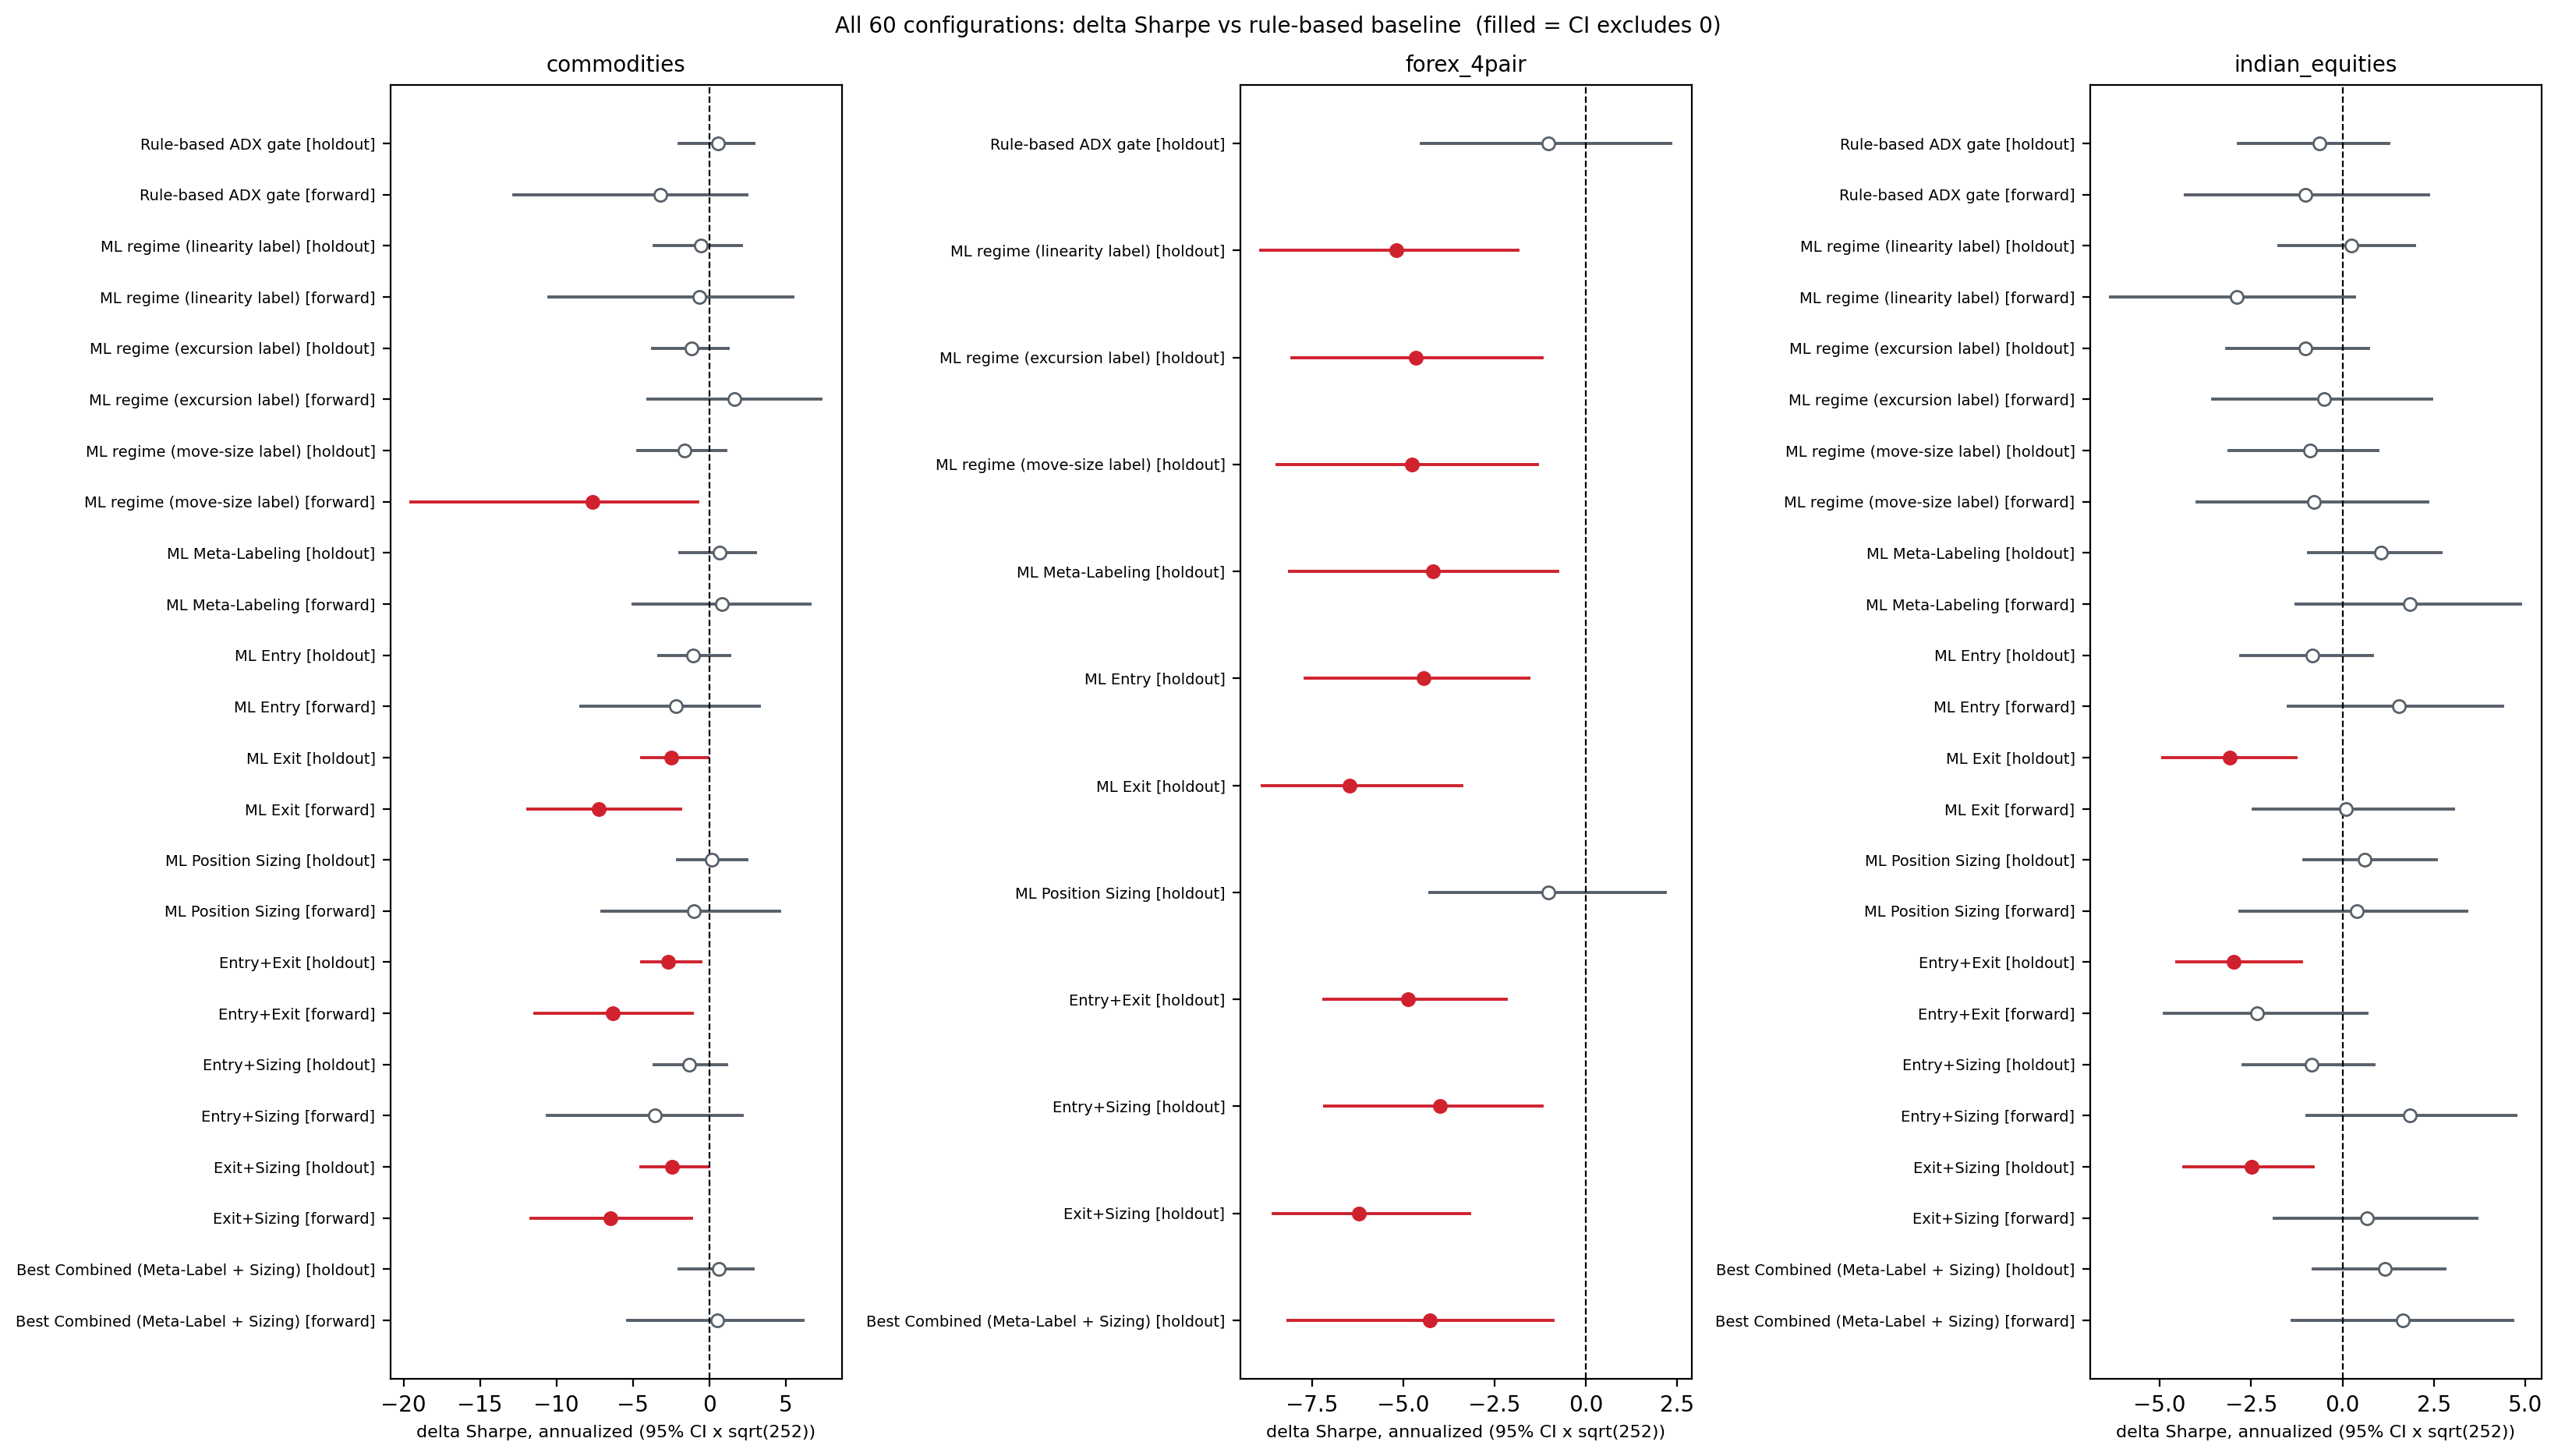
\includegraphics[width=\textwidth]{figures/p36_fig1_component_attribution_forest.png}
  \caption{All 60 configurations, forest plot with 95\% bootstrap CIs, one panel per market. Dots
  are annualized $\Delta$Sharpe; intervals are the per-day bootstrap CIs rescaled by $\sqrt{252}$ so
  both share one axis (earlier drafts drew the unscaled per-day interval around the annualized
  point; significance calls are unaffected). Filled = CI excludes zero.}
  \label{fig:attribution_forest}
\end{figure*}

\subsection{Independent components: the regime filter}

The regime filter is a dead end everywhere tested. All three ML label variants (linearity,
excursion, move-size) lose against the rule-based ADX gate's own already-weak baseline in every
market; one configuration (move-size label, commodities forward) loses significantly.
\textbf{Why:} an independent gate can only reject bars; it cannot compensate for a weak or noisy
label definition by learning from the entry signal itself, since it never sees it. The rule-based
ADX gate this component is meant to improve on already underperforms not gating at all on these
three markets (a pre-ML finding this repository established before any ML work began), so an ML
variant of a rule that itself adds little has little to inherit.

\subsection{Narrowing components: meta-labeling and position sizing}

Meta-labeling and position sizing show the only encouraging (still non-significant) pattern in the
entire campaign, concentrated in Indian equities: both beat baseline on holdout and forward Sharpe
there (Meta-Labeling: $\Delta$Sharpe +1.04 holdout, +1.84 forward; Position Sizing: +0.60 holdout,
+0.38 forward). Position sizing --- the identical underlying win-probability model, consumed as a
continuous multiplier rather than a threshold --- replicates the same directional pattern with a
smaller effect size. \textbf{Why:} both components can only subtract from or re-weight the
rule-based system's own trade set; they cannot invent new entries or exits, which bounds their
downside relative to the replacing components below. Forex is again the exception: meta-labeling
loses significantly there (the only significant loss either narrowing component produces).

\subsection{Replacing components: entry and exit}

\textbf{Entry.} ML Entry loses on forex (significantly), is mixed on commodities, and is marginally
positive but non-significant on Indian equities. \textbf{Why:} entry replacement discards the
rule-based JMA crossover's own trend-detection logic entirely and asks a classifier to rediscover
it from the same 8 features with no lookahead advantage; on forex, where the rule-based baseline
already achieves the campaign's highest Sharpe (5.53 on holdout), there is apparently little signal
left for a learned entry model to find, and every departure from the rule looks like noise.

\textbf{Exit.} ML Exit is the clearest, most consistent failure mode of any single component: it
loses significantly in 4 of 5 tested configurations. \textbf{Why, mechanistically, not just
observationally:} trade count inflates 2.7$\times$--4.2$\times$ across every market, because an
exit that fires sooner than the rule-based ATR bracket un-blocks bars that a longer-held baseline
trade would have absorbed, letting intervening JMA crossovers become their own separate, smaller,
fee-eaten trades. This is a structural property of replacing a \emph{holding} mechanism (a bracket
that commits capital for a variable duration) with a per-bar \emph{continuation classifier} that
re-evaluates every bar independently --- not a symptom of an undertrained or mistuned model.

\textbf{Effect size scales with how much a component can alter the realized trade set,} consistent
with the Section~\ref{sec:taxonomy} taxonomy's ex-ante hypothesis: position sizing (never rejects a
trade) does the least damage; meta-labeling (rejects trades, keeps entry/exit fixed) is more
volatile; entry and exit replacement (discard the rule-based mechanism outright) produce the
largest swings, almost always negative.

\subsection{Statistical validation}

Every $\Delta$Sharpe carries a 95\% bootstrap CI (2{,}000 replicates; Section~\ref{sec:methodology}), and
every Sharpe is reported alongside its deflated Sharpe ratio, correcting for the actual number of
variants screened within that component. No pooled cross-market or cross-component test is
attempted: markets have too few instruments (4--48) and components too few evaluation windows for
a meaningful meta-analytic pooling beyond the descriptive Opportunity Matrix itself;
Section~\ref{sec:limitations} discusses multiple-comparisons handling in more detail.

\section{Combinations}
\label{sec:combinations}

Four combination experiments, run under the identical freeze/holdout/forward protocol and
frozen-model-reuse discipline as every individual component: (1) \textbf{Entry+Exit} --- ML Entry's
signal generation feeding ML Exit's continuation-based exit mechanism; (2) \textbf{Entry+Sizing}
--- ML Entry generating trades, ML Position Sizing re-weighting them; (3) \textbf{Exit+Sizing} ---
rule-based entry, ML Exit's exit mechanism, ML Position Sizing re-weighting; (4) \textbf{Best
Combined} --- chosen empirically, not assumed in advance: ML Meta-Labeling composed with ML
Position Sizing, the two \emph{narrowing} components that individually showed the paper's only
encouraging pattern (Section~\ref{sec:taxonomy}).

\begin{longtable}{l l l r r r r l}
\caption{Combination experiments: 4 combinations $\times$ 3 markets $\times$ available windows (20 configurations).} \label{tab:combinations} \\
\toprule
Market & Window & Variant & Trades & Sharpe (base $\to$ variant) & Deflated Sharpe & $\Delta$Sharpe & Significant? \\
\midrule
\endhead
\bottomrule
\endfoot
commodities & forward & best\_combined & 37 & 4.17 $\to$ 4.67 & 0.997 & +0.49 & no \\
commodities & forward & entry\_exit & 210 & 4.17 $\to$ -2.14 & 0.106 & -6.31 & \textbf{yes} \\
commodities & forward & entry\_sizing & 65 & 4.17 $\to$ 0.62 & 0.619 & -3.55 & no \\
commodities & forward & exit\_sizing & 113 & 4.17 $\to$ -2.28 & 0.123 & -6.45 & \textbf{yes} \\
commodities & holdout & best\_combined & 170 & 2.72 $\to$ 3.34 & 1.000 & +0.61 & no \\
commodities & holdout & entry\_exit & 1420 & 2.72 $\to$ 0.05 & 0.618 & -2.68 & \textbf{yes} \\
commodities & holdout & entry\_sizing & 335 & 2.72 $\to$ 1.40 & 0.957 & -1.33 & no \\
commodities & holdout & exit\_sizing & 610 & 2.72 $\to$ 0.30 & 0.723 & -2.42 & \textbf{yes} \\
forex\_4pair & holdout & best\_combined & 118 & 5.53 $\to$ 1.26 & 0.831 & -4.27 & \textbf{yes} \\
forex\_4pair & holdout & entry\_exit & 1233 & 5.53 $\to$ 0.66 & 0.977 & -4.88 & \textbf{yes} \\
forex\_4pair & holdout & entry\_sizing & 243 & 5.53 $\to$ 1.54 & 0.966 & -3.99 & \textbf{yes} \\
forex\_4pair & holdout & exit\_sizing & 596 & 5.53 $\to$ -0.68 & 0.321 & -6.21 & \textbf{yes} \\
indian\_equities & forward & best\_combined & 197 & 1.05 $\to$ 2.70 & 0.994 & +1.65 & no \\
indian\_equities & forward & entry\_exit & 1794 & 1.05 $\to$ -1.29 & 0.089 & -2.34 & no \\
indian\_equities & forward & entry\_sizing & 290 & 1.05 $\to$ 2.89 & 0.999 & +1.83 & no \\
indian\_equities & forward & exit\_sizing & 915 & 1.05 $\to$ 1.73 & 0.991 & +0.68 & no \\
indian\_equities & holdout & best\_combined & 527 & 2.84 $\to$ 4.01 & 1.000 & +1.16 & no \\
indian\_equities & holdout & entry\_exit & 3420 & 2.84 $\to$ -0.13 & 0.586 & -2.97 & \textbf{yes} \\
indian\_equities & holdout & entry\_sizing & 756 & 2.84 $\to$ 2.00 & 1.000 & -0.84 & no \\
indian\_equities & holdout & exit\_sizing & 1279 & 2.84 $\to$ 0.36 & 0.773 & -2.48 & \textbf{yes} \\
\end{longtable}


\begin{figure*}[h]
  \centering
  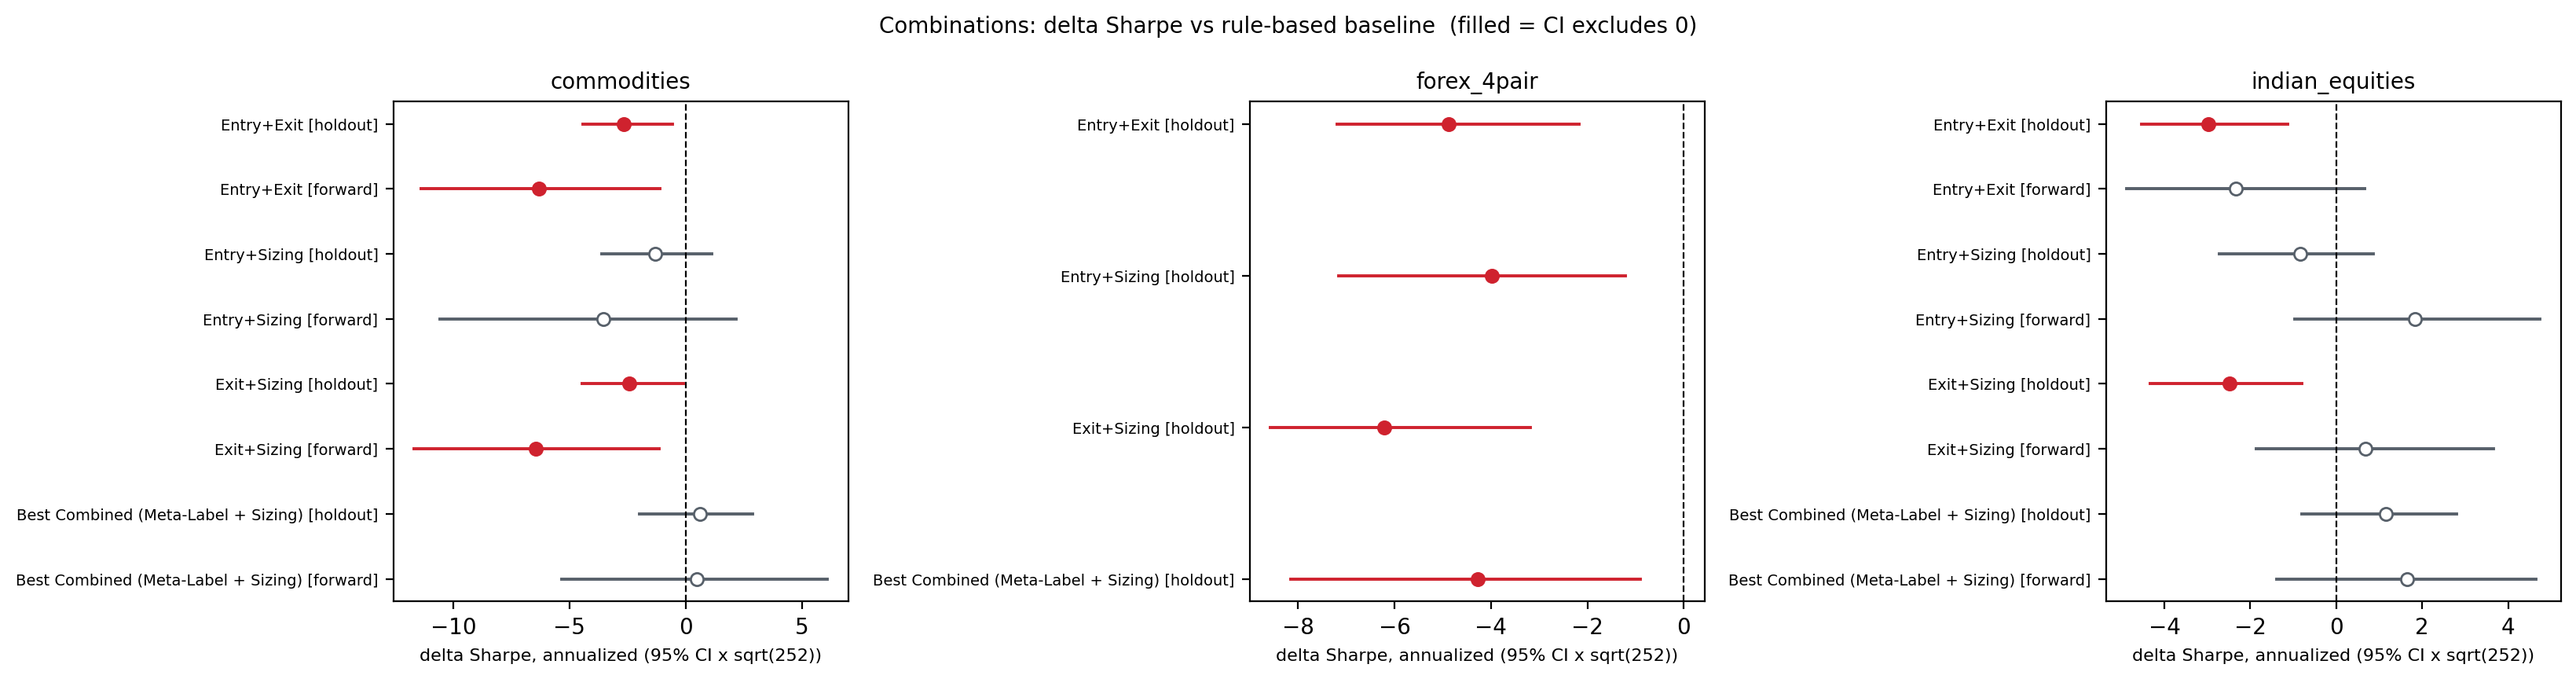
\includegraphics[width=\textwidth]{figures/p36_fig2_combinations_forest.png}
  \caption{The 20 combination-only rows, same convention as Figure~\ref{fig:attribution_forest}.}
  \label{fig:combinations_forest}
\end{figure*}

\textbf{Any combination containing ML Exit inherits its overtrading failure, and composition does
not average it away.} Entry+Exit and Exit+Sizing both explode trade count and both lose,
significantly on 6 of 8 testable holdout/forward pairs. Composing ML Exit with a component that
individually looked fine (Position Sizing) does not rescue it --- consistent with the
turnover-inflation mechanism identified above being a property of the exit mechanism itself, not
something a downstream narrowing component can correct after the fact.

\textbf{Entry+Sizing is gentler than ML Entry alone,} consistent with a dose-response reading:
position sizing can only re-weight the trades ML Entry generates, not reject them, so it softens
but does not reverse ML Entry's forex loss, and turns indian\_equities forward strongly positive
(1.05 $\to$ 2.89), though the CI still touches zero.

\textbf{Best Combined --- composing two narrowing components --- is the campaign's standout
result, and still falls short of significance.} Indian-equities holdout Sharpe improves from 2.84
to 4.01 with a bootstrap CI of $[-0.050, 0.176]$, the closest any of the 60 tested configurations
comes to excluding zero. Forex remains the exception: Best Combined still loses there
significantly, reinforcing that forex is hostile to the mechanism itself, not merely to any one
component's implementation.

\textbf{Composition amplifies a shared directional pattern rather than creating value the
individual components lacked.} Best Combined's indian\_equities holdout Sharpe (4.01) exceeds both
Meta-Labeling alone (3.89) and Position Sizing alone (3.44), suggesting the two narrowing
components' gains are at least partially additive here --- consistent with the taxonomy prediction
that narrowing components address different axes of the same decision (which trades to keep, vs.\
how much to risk on them) and so do not simply duplicate each other's effect. This is, however, a
single freeze-date observation (Section~\ref{sec:limitations}).

\section{Discussion}
\label{sec:discussion}

\subsection{What MBCA reveals}

Across 60 tested configurations, zero showed a statistically significant improvement over the
rule-based baseline, even when the two most promising components were composed together. Read at
face value, this could suggest ``ML does not help hybrid trading systems.'' MBCA's contribution is
to show that this framing is both too strong and not useful: the honest reading is narrower and
more actionable. ML's contribution here is component-specific and market-specific, and the
Section~\ref{sec:taxonomy} taxonomy predicts much of that heterogeneity ex ante: narrowing
components (which can only subtract or re-weight) are gentler and occasionally directionally
positive; replacing components (which can generate an entirely different trade set) are more
volatile and, for exit specifically, actively harmful via an identified turnover mechanism that
propagates into any combination containing it; and the one independent component tested, the
regime filter, is a dead end everywhere, inheriting the weakness of the rule-based gate it was
meant to improve on.

\subsection{Why forex is different}

Forex is hostile to every ML intervention and every combination tested: every configuration on
that sleeve loses on holdout, and most losses are statistically significant. One plausible
explanation is that the rule-based 4-pair JMA+ATR recipe already extracts most of the value
available in this feature set on this sleeve --- its own rule-based holdout Sharpe (5.53) is the
highest of any market's baseline in this study --- leaving little residual signal for a learned
model, at this feature budget, to find. Every departure from the rule, in this reading, looks like
noise rather than an improvement. This is a hypothesis consistent with the pattern, not something
we can prove definitively from a single freeze date; the alternative explanation --- that this
particular feature set or model class is simply mismatched to forex specifically --- cannot be
ruled out from this evidence alone (Section~\ref{sec:limitations}). The independent replication
(Section~\ref{sec:replication}) weakens this finding further: with different forex data and a flat
cost model, the rule-based baseline is much weaker and only 2 of 12 forex configurations lose
significantly, so ``forex is hostile to ML'' should be read as specific to the original data and cost
setup.

\subsection{Why composition amplifies rather than creates}

Composing two individually-non-negative components (Best Combined) amplifies their shared
directional pattern --- Indian-equities holdout Sharpe reaches 4.01, above either component alone
--- rather than cancelling it. But amplification of a non-significant effect is still
non-significant. This is a useful negative result in its own right: it means the near-miss is not
an artifact of noise in one component being fortuitously offset by noise in another (which would
predict regression toward zero on composition), but a case where two components pointing the same
direction reinforce each other. That reinforcement pattern is itself evidence the underlying
signal, while too small to call significant at this sample size, is not pure noise --- which is
precisely why we flag Best Combined, and not any other configuration, as the single one worth a
second-freeze-date replication.

\subsection{Toward MBCA beyond trading}

We designed and applied MBCA to one trading strategy because it gave us an already-validated
rule-based control and a market structure (three distinct markets) that let us test whether
component-level patterns generalize across data-generating processes without changing the
pipeline. Nothing in MBCA's definition (Section~\ref{sec:mbca}) is trading-specific: it applies
wherever a system combines a rule-based or otherwise validated control with candidate learned
components at distinct decision points --- for instance, control systems that combine PID
controllers with learned correction terms, recommendation pipelines that combine heuristic ranking
with learned re-ranking stages, or clinical decision-support tools that combine guideline-based
triage with learned risk scores. We propose this as a direction, not a demonstrated result: this
paper tests MBCA on one domain, and we have not run it on a non-trading system.
Section~\ref{sec:future} lists this as the most valuable extension for establishing MBCA's
generality beyond the claim we can support here.

\subsection{Practical implications}

For practitioners with an already-validated rule-based system, this evidence
(Figure~\ref{fig:matrix}, Figure~\ref{fig:decision}) suggests: skip an independent regime-filter
gate unless the underlying rule-based gate itself has separately demonstrated value; prioritize
narrowing components (meta-labeling, position sizing) over replacing components when adding ML,
particularly in markets showing structural regime shifts (Indian equities, in this study); avoid
learned entry/exit replacement, since the rule-based mechanism appears to already be near-optimal,
or the replacement introduces new failure modes (turnover inflation), given this feature/model
budget; and treat any positive, non-significant result --- including Best Combined --- as
exploratory until replicated at a second, independent freeze date.

\begin{figure*}[h]
  \centering
  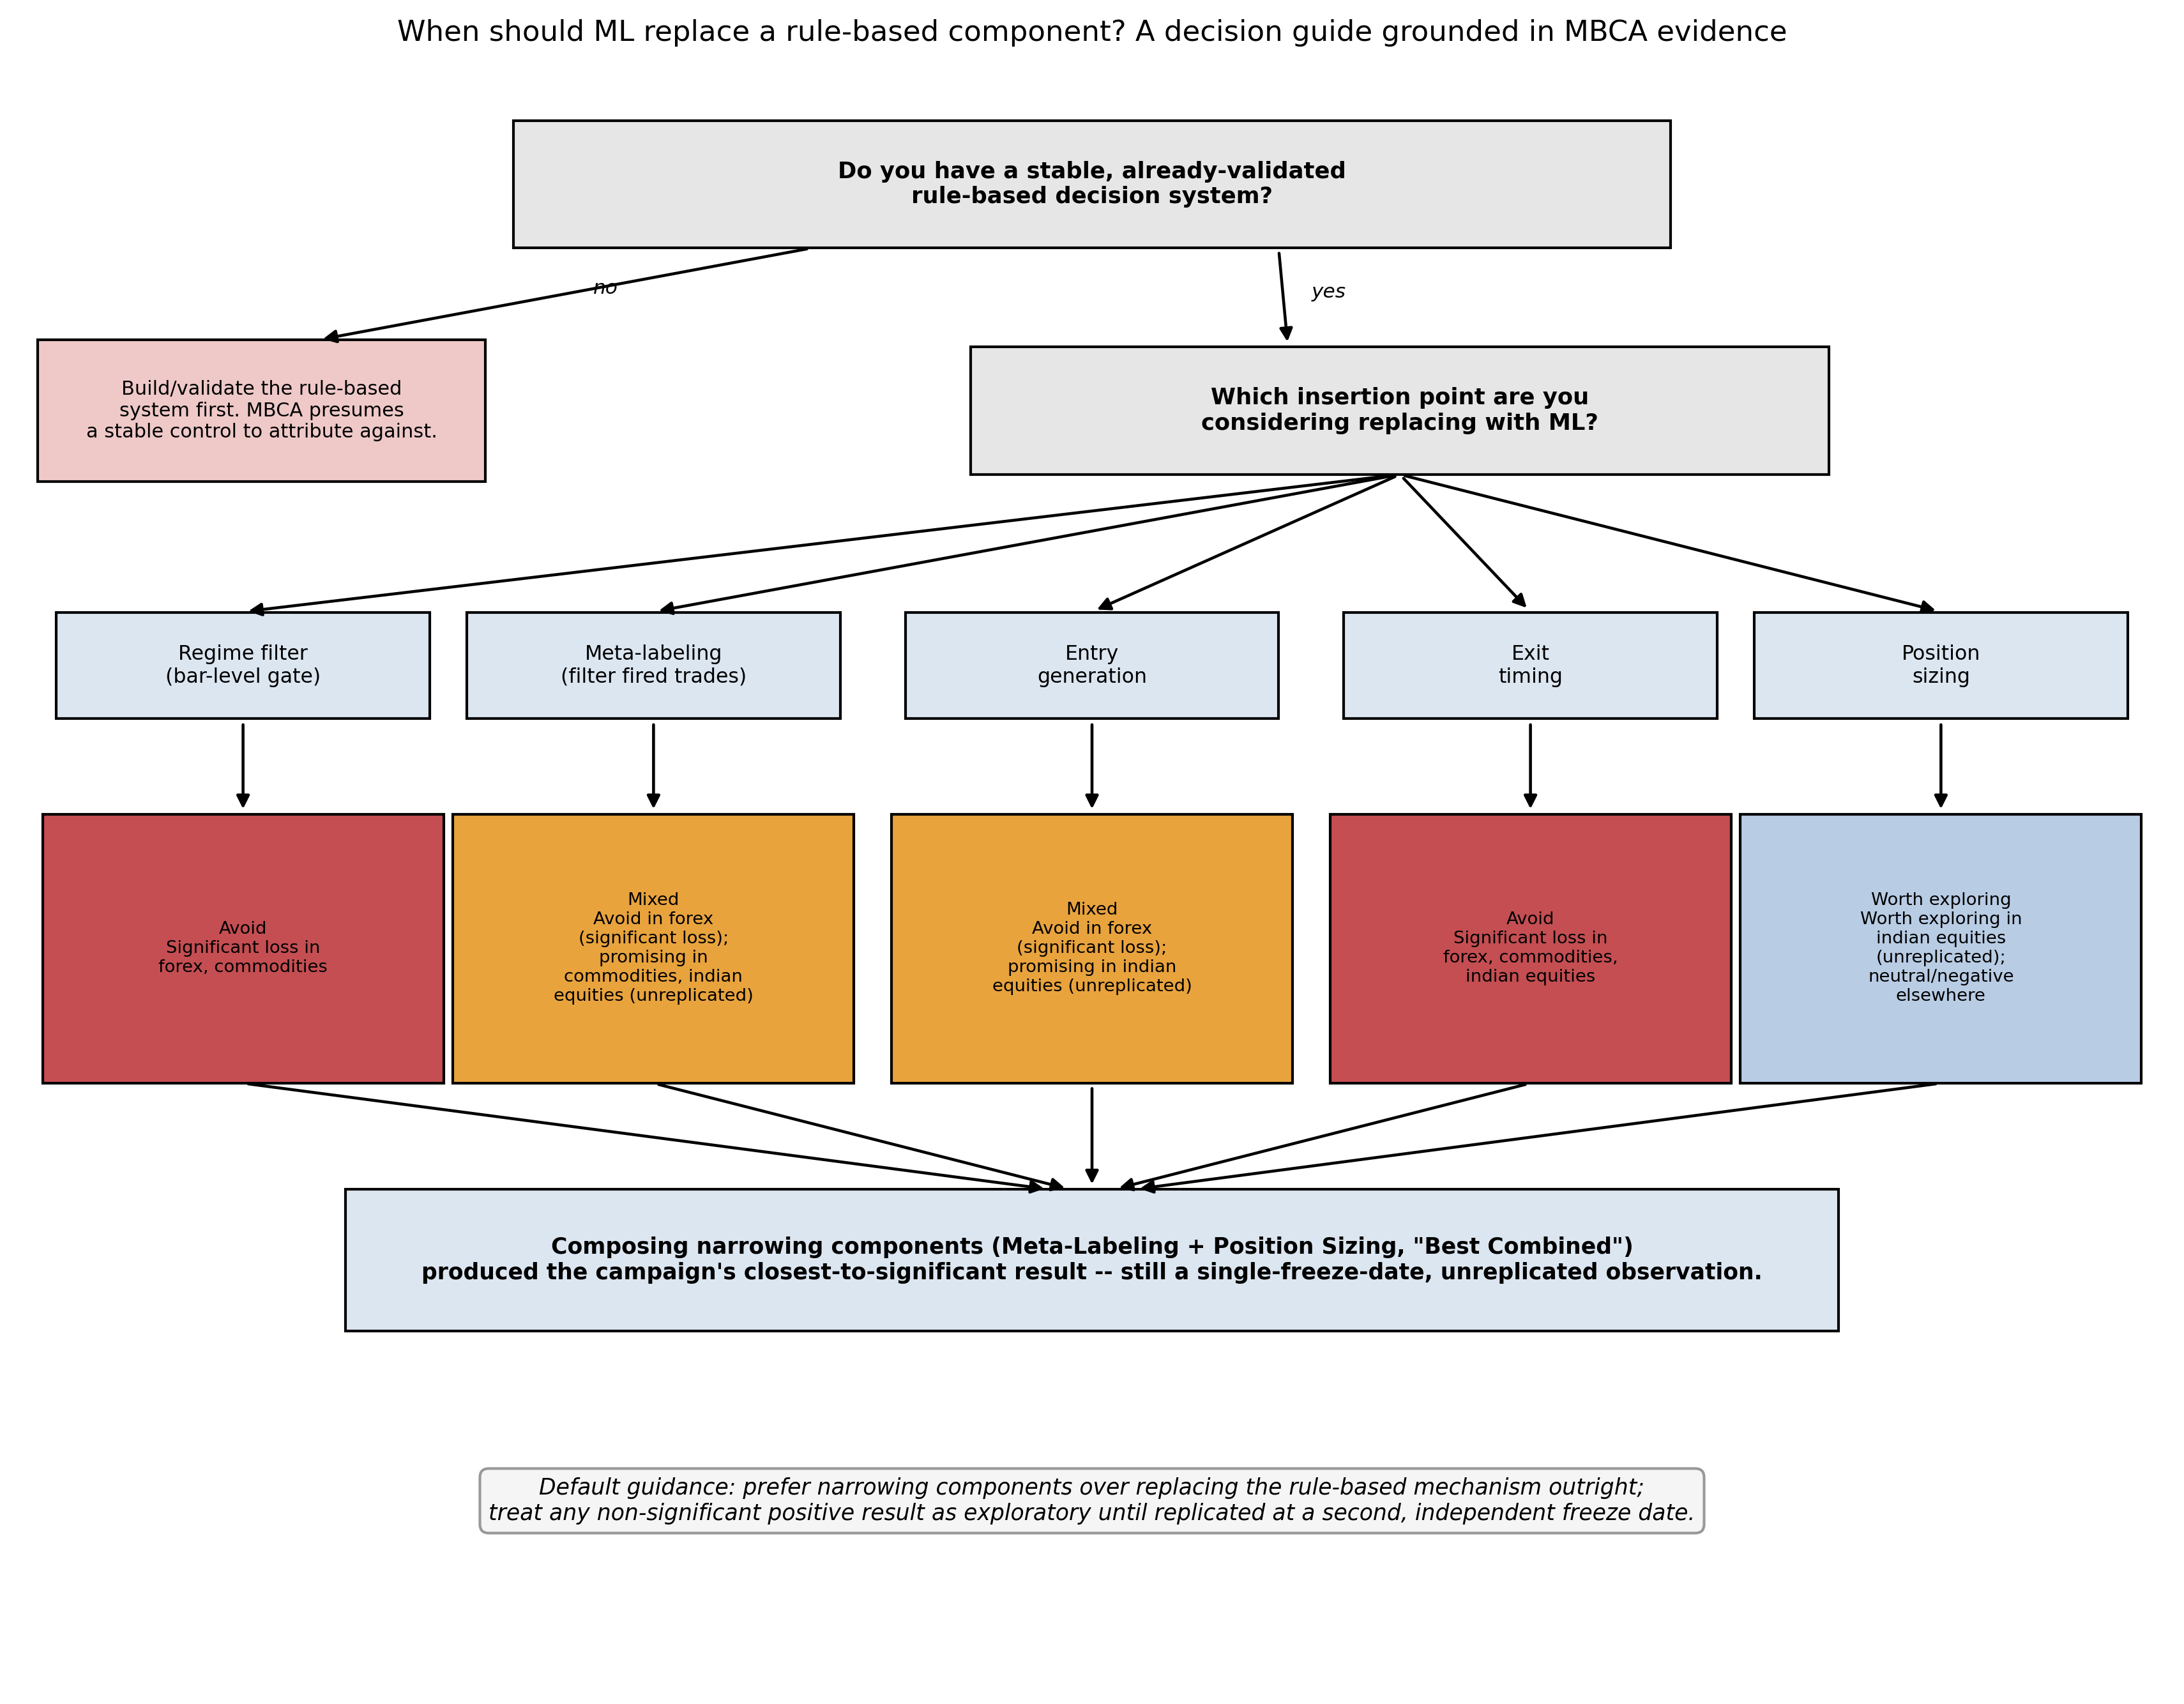
\includegraphics[width=\textwidth]{figures/p36_fig_decision_flowchart.png}
  \caption{A decision guide for whether to convert a given insertion point to ML, grounded directly
  in the Section~\ref{sec:results}--\ref{sec:combinations} evidence; every leaf reuses the same
  mechanically-derived recommendation shown in Figure~\ref{fig:matrix}.}
  \label{fig:decision}
\end{figure*}

\section{Limitations}
\label{sec:limitations}

We address five objections directly, in order of severity.

\begin{itemize}
  \item \textbf{Every result is a single freeze-date observation per market.} This is the paper's
        most serious limitation. No component/market pairing --- individual or combined --- has
        been replicated at a second, independent split point. It applies with particular force to
        Best Combined's near-miss result in Indian equities (bootstrap CI $[-0.050, 0.176]$): a
        single-freeze-date confidence interval that happens to sit close to excluding zero is not
        evidence of a real effect on its own, and we do not treat it as one. We report it as the
        single configuration most worth a second-freeze-date replication
        (Section~\ref{sec:future}), not as a validated finding.
  \item \textbf{One feature set, one model class.} This is deliberate, and it is the point of
        MBCA, not an oversight: sweeping features or hyperparameters per component would confound
        component differences with tuning-effort differences, which is exactly the confound MBCA
        is designed to eliminate (Section~\ref{sec:mbca}). But this means every negative result in
        this paper is a statement about \emph{this specific budget} at that insertion point --- 8
        backward-only features, one LightGBM configuration --- not a universal claim that no
        learned policy could ever add value there. A different feature set (e.g.\ market
        microstructure, alternative data) or model class might change individual results; MBCA's
        contribution is the protocol for testing that fairly, not a claim that this paper has
        exhausted the space of possible ML configurations at each insertion point.
  \item \textbf{No calibration analysis.} We report trading-performance metrics (Sharpe, CAGR,
        drawdown, deflated Sharpe, bootstrap CI) throughout; we do not report classifier
        calibration metrics (Brier score, expected calibration error, reliability diagrams) for
        any component's underlying classifier. This is a scope decision, not an oversight, and we
        do not claim otherwise: a well-calibrated classifier can still produce a
        poorly-performing trading component (if its features carry little signal), and a
        poorly-calibrated one can still trade profitably (if its rank-ordering is useful even when
        its probabilities are not). Calibration analysis is a natural, separate extension
        (Section~\ref{sec:future}), not a claim we make here.
  \item \textbf{Multiple-comparisons handling.} Each Sharpe is reported alongside a deflated Sharpe
        ratio that corrects for the number of variants screened \emph{within that component's own
        campaign} (e.g.\ \texttt{n\_trials=3} for the Regime Filter's three label variants). We do
        not apply a single global correction (e.g.\ Bonferroni) across all 60 tested
        configurations, because the paper's claim is component-specific and market-specific, not a
        claim that ML generally helps trading. A reader who prefers a fully conservative,
        globally-corrected reading should treat every non-significant result in this paper
        (including Best Combined) as, if anything, more exploratory still --- our own framing
        already treats it that way.
  \item \textbf{Matched-budget fairness.} A natural objection: forcing every component to share
        identical hyperparameters might handicap components that would benefit from different
        tuning. We accept this trade-off explicitly, because the alternative --- tuning each
        component separately --- answers a different question (``which component performs best
        given unlimited tuning effort'') than the one MBCA is designed to answer (``holding effort
        fixed, where does ML add value''). Per-component hyperparameter sensitivity is listed as
        future work (Section~\ref{sec:future}), not folded into this paper's headline claims.
\end{itemize}

Two further, narrower limitations carry over from the underlying strategy validation:
\begin{itemize}
  \item \textbf{Forex has no forward tree} --- holdout-only evidence for that market.
  \item \textbf{Crypto was not included} --- no equivalent pre-ML validated baseline or
        forward-tail tree exists yet for that market; this is a scope limitation, not a null
        result.
  \item \textbf{No claim of a validated, deployable trading strategy.} Nothing here is
        paper-traded, and no positive trading-performance claim is made.
\end{itemize}

\section{Future Work: Extending MBCA}
\label{sec:future}

\begin{itemize}
  \item \textbf{Second, independent freeze-date replication} per market, prioritizing Best
        Combined (Meta-Labeling + Position Sizing) in Indian equities first --- the single most
        valuable next step, since it is the one configuration whose current evidence is closest to
        informative.
  \item \textbf{Extend the component-attribution protocol to crypto} once an equivalent pre-ML
        validated baseline and forward-tail tree exist.
  \item \textbf{Test MBCA on a non-trading hybrid system} (e.g.\ a rule-based control loop with a
        learned correction term, or a heuristic ranking pipeline with a learned re-ranking stage)
        to establish whether the taxonomy and matrix format proposed in
        Section~\ref{sec:discussion} generalize beyond trading, which this paper does not itself
        demonstrate.
  \item \textbf{Classifier calibration analysis} (Brier score, reliability diagrams) per
        component, to test whether calibration quality predicts which components are worth
        converting to ML independent of realized trading performance.
  \item \textbf{Alternative budgets:} investigate whether a minimum-hold-bars floor or a
        K-consecutive-signal exit rule removes ML Exit's turnover-inflation failure mode, and
        whether this rescues Entry+Exit/Exit+Sizing; and whether a different feature set or model
        class changes which components fall into which taxonomy bucket.
  \item \textbf{Shared model refit:} test the Best Combined pairing against a shared, jointly-fit
        meta-label model rather than the campaign's current independent refit inside
        \texttt{PositionSizeModel}, to rule out any avoidable variance in the near-miss result.
\end{itemize}

\section{Reference Implementation and Independent Replication}
\label{sec:replication}

We release \texttt{mbca}, a self-contained Python package (pandas, scikit-learn, LightGBM) that
implements MBCA end to end: the eight shared features, the rule-based pipeline and walk-forward
harness, the five components as drop-in replacements of one pipeline function each, the freeze
protocol, and the statistics of Section~\ref{sec:methodology}. Its test suite enforces the paper's
methodological invariants directly: features computed on data truncated at bar $t$ equal those
computed on the full series (no lookahead); scrambling every post-split bar leaves every fitted model
bit-for-bit unchanged (freeze); position sizing never adds or removes a trade; and components compose
by replacing exactly one insertion point. A user supplies their own entry rule, exit rule, and data,
and obtains the full attribution table and Opportunity Matrix for their strategy.

Because \texttt{mbca} was written from scratch rather than copied from the study pipeline, re-running
the full 60-configuration grid with it is an independent replication, with three known differences:
the forex data come from a different vendor with a flat 7\,bps cost instead of per-pair spread and
swap; Indian equities are traded without the annual sector-curation overlay; and one walk-forward
over the full history replaces the separately-fetched forward tree. Table~\ref{tab:replication}
compares every configuration.

\begin{longtable}{l l l r r l l}
\caption{Paper vs.\ independent replication (\texttt{mbca}), $\Delta$Sharpe (annualized) per configuration.} \label{tab:replication} \\
\toprule
Market & Window & Variant & Paper & Replication & Paper verdict & Replication verdict \\
\midrule
\endhead
\bottomrule
\endfoot
commodities & forward & Rule-based ADX gate & -3.23 & -5.03 & n.s. & n.s. \\
commodities & forward & ML Regime Filter (linearity) & -0.67 & -3.51 & n.s. & n.s. \\
commodities & forward & ML Regime Filter (excursion) & +1.63 & +2.13 & n.s. & n.s. \\
commodities & forward & ML Regime Filter (move\_size) & -7.65 & +1.63 & sig.\ loss & n.s. \\
commodities & holdout & Rule-based ADX gate & +0.54 & +0.51 & n.s. & n.s. \\
commodities & holdout & ML Regime Filter (linearity) & -0.54 & +2.19 & n.s. & n.s. \\
commodities & holdout & ML Regime Filter (excursion) & -1.16 & +0.20 & n.s. & n.s. \\
commodities & holdout & ML Regime Filter (move\_size) & -1.65 & -0.81 & n.s. & n.s. \\
forex & holdout & Rule-based ADX gate & -1.02 & -1.05 & n.s. & n.s. \\
forex & holdout & ML Regime Filter (linearity) & -5.20 & -0.02 & sig.\ loss & n.s. \\
forex & holdout & ML Regime Filter (excursion) & -4.66 & -3.55 & sig.\ loss & n.s. \\
forex & holdout & ML Regime Filter (move\_size) & -4.78 & -2.16 & sig.\ loss & n.s. \\
indian\_equities & forward & Rule-based ADX gate & -1.01 & -0.43 & n.s. & n.s. \\
indian\_equities & forward & ML Regime Filter (linearity) & -2.89 & -0.21 & n.s. & n.s. \\
indian\_equities & forward & ML Regime Filter (excursion) & -0.51 & -0.43 & n.s. & n.s. \\
indian\_equities & forward & ML Regime Filter (move\_size) & -0.78 & +0.29 & n.s. & n.s. \\
indian\_equities & holdout & Rule-based ADX gate & -0.63 & -1.39 & n.s. & n.s. \\
indian\_equities & holdout & ML Regime Filter (linearity) & +0.23 & -1.35 & n.s. & n.s. \\
indian\_equities & holdout & ML Regime Filter (excursion) & -1.01 & -1.27 & n.s. & n.s. \\
indian\_equities & holdout & ML Regime Filter (move\_size) & -0.89 & -1.69 & n.s. & sig.\ loss \\
commodities & forward & ML Meta-Labeling & +0.83 & -0.47 & n.s. & n.s. \\
commodities & holdout & ML Meta-Labeling & +0.67 & +1.27 & n.s. & n.s. \\
forex & holdout & ML Meta-Labeling & -4.19 & +0.94 & sig.\ loss & n.s. \\
indian\_equities & forward & ML Meta-Labeling & +1.84 & +1.40 & n.s. & n.s. \\
indian\_equities & holdout & ML Meta-Labeling & +1.04 & -0.02 & n.s. & n.s. \\
commodities & forward & ML Entry & -2.17 & -3.50 & n.s. & n.s. \\
commodities & holdout & ML Entry & -1.06 & -0.12 & n.s. & n.s. \\
forex & holdout & ML Entry & -4.46 & -1.06 & sig.\ loss & n.s. \\
indian\_equities & forward & ML Entry & +1.53 & +0.37 & n.s. & n.s. \\
indian\_equities & holdout & ML Entry & -0.82 & -1.86 & n.s. & sig.\ loss \\
commodities & forward & ML Exit & -7.22 & -6.16 & sig.\ loss & sig.\ loss \\
commodities & holdout & ML Exit & -2.47 & -1.61 & sig.\ loss & n.s. \\
forex & holdout & ML Exit & -6.48 & -3.87 & sig.\ loss & sig.\ loss \\
indian\_equities & forward & ML Exit & +0.09 & -0.12 & n.s. & n.s. \\
indian\_equities & holdout & ML Exit & -3.08 & -5.07 & sig.\ loss & sig.\ loss \\
commodities & forward & ML Position Sizing & -1.04 & -1.13 & n.s. & n.s. \\
commodities & holdout & ML Position Sizing & +0.16 & +0.18 & n.s. & n.s. \\
forex & holdout & ML Position Sizing & -1.03 & -0.79 & n.s. & n.s. \\
indian\_equities & forward & ML Position Sizing & +0.38 & +0.18 & n.s. & n.s. \\
indian\_equities & holdout & ML Position Sizing & +0.60 & +0.16 & n.s. & n.s. \\
commodities & forward & Entry+Exit & -6.31 & -7.19 & sig.\ loss & sig.\ loss \\
commodities & forward & Entry+Sizing & -3.55 & -5.86 & n.s. & sig.\ loss \\
commodities & forward & Exit+Sizing & -6.45 & -5.45 & sig.\ loss & sig.\ loss \\
commodities & forward & Best Combined (Meta-Label + Sizing) & +0.49 & -0.93 & n.s. & n.s. \\
commodities & holdout & Entry+Exit & -2.68 & -1.66 & sig.\ loss & n.s. \\
commodities & holdout & Entry+Sizing & -1.33 & -0.34 & n.s. & n.s. \\
commodities & holdout & Exit+Sizing & -2.42 & -1.31 & sig.\ loss & n.s. \\
commodities & holdout & Best Combined (Meta-Label + Sizing) & +0.61 & +1.19 & n.s. & n.s. \\
forex & holdout & Entry+Exit & -4.88 & -3.34 & sig.\ loss & n.s. \\
forex & holdout & Entry+Sizing & -3.99 & -0.93 & sig.\ loss & n.s. \\
forex & holdout & Exit+Sizing & -6.21 & -3.91 & sig.\ loss & sig.\ loss \\
forex & holdout & Best Combined (Meta-Label + Sizing) & -4.27 & +1.11 & sig.\ loss & n.s. \\
indian\_equities & forward & Entry+Exit & -2.34 & -2.44 & n.s. & n.s. \\
indian\_equities & forward & Entry+Sizing & +1.83 & +0.36 & n.s. & n.s. \\
indian\_equities & forward & Exit+Sizing & +0.68 & +0.40 & n.s. & n.s. \\
indian\_equities & forward & Best Combined (Meta-Label + Sizing) & +1.65 & +1.53 & n.s. & n.s. \\
indian\_equities & holdout & Entry+Exit & -2.97 & -5.02 & sig.\ loss & sig.\ loss \\
indian\_equities & holdout & Entry+Sizing & -0.84 & -2.13 & n.s. & sig.\ loss \\
indian\_equities & holdout & Exit+Sizing & -2.48 & -4.39 & sig.\ loss & sig.\ loss \\
indian\_equities & holdout & Best Combined (Meta-Label + Sizing) & +1.16 & +0.04 & n.s. & n.s. \\
\end{longtable}


\textbf{What replicates.} (i) Zero of 60 configurations show a significant improvement, in the
paper and in the replication. (ii) 49 of 60 configurations agree in the sign of $\Delta$Sharpe.
(iii) ML Exit is the most reliably harmful component: significant losses in all three markets,
with trade count inflated 2.4--3.0$\times$ (paper: 2.7--4.2$\times$) --- the turnover mechanism of
Section~\ref{sec:results} reappears in an independent implementation. (iv) Every combination
containing ML Exit loses in 9 of 10 holdout/forward configurations in both runs. (v) The narrowing
components remain the only ones directionally positive in more than one market.

\textbf{What does not.} (i) \emph{Forex hostility is not robust.} The paper found significant losses
in 10 of 12 forex configurations; the replication finds 2 of 12 (ML Exit and Exit+Sizing), and
Meta-Labeling flips from $-4.19$ to $+0.94$. The rule-based forex baseline is also far weaker
(holdout Sharpe 1.39 vs.\ 5.53), consistent with Section~\ref{sec:discussion}'s hypothesis that ML
looked hostile on forex because the baseline left little residual signal --- a hypothesis that
depends on the data vendor and cost model, not only on the market. (ii) \emph{Best Combined's
near-miss is only half replicated.} Its Indian-equities forward improvement reproduces closely
($+1.53$ vs.\ $+1.65$, CI $[-0.051, 0.251]$), but the holdout improvement does not ($+0.04$ vs.\
$+1.16$) once the sector-curation overlay is removed and the baseline itself rises to 4.31. (iii)
The replication finds 12 significant losses rather than 20, mostly because of the forex difference.

\textbf{Reading.} The conclusions this paper draws at the level of the \emph{method} and the
\emph{taxonomy} --- no ML component significantly improves a validated rule-based system at this
budget; replacing a holding mechanism with a per-bar continuation classifier is structurally harmful;
narrowing components are the only candidates worth further study --- survive an independent
re-implementation. Conclusions at the level of a specific market or a specific configuration's
effect size do not survive reliably, and we have weakened the corresponding claims above
accordingly. This is the discipline MBCA recommends to its users: treat per-cell effects as
exploratory until replicated.

\section{Conclusion}

We introduced Matched-Budget Component Attribution (MBCA), a controlled-variable methodology for
deciding where, specifically, a machine-learned component adds value inside an already-validated
hybrid decision system. MBCA holds data, features, model class, freeze discipline, and evaluation
protocol fixed and varies only the insertion point, so that a resulting performance delta can be
attributed to that insertion point rather than to a confound of tuning or feature-engineering
effort.

Applying MBCA to one rule-based trading system across three markets and 60 configurations (5
components, 4 combinations, up to 2 evaluation windows each), we found zero statistically
significant improvements and twenty statistically significant losses, concentrated in the forex
sleeve and the ML Exit component (a turnover-inflation failure mode identified and explained, not
just observed, and inherited rather than averaged away by any combination containing it). A
taxonomy of insertion points --- independent, narrowing, replacing --- predicted much of this
heterogeneity ex ante: narrowing components (meta-labeling, position sizing) showed a mild,
market-concentrated, non-significant positive pattern, while replacing components (entry, exit)
were more volatile and often actively harmful. The one genuinely encouraging signal, Best Combined
(Meta-Labeling filtering trades, then Position Sizing re-weighting the survivors), came closer to
statistical significance in Indian equities (bootstrap CI $[-0.050, 0.176]$) than any other
configuration tested, beat baseline on both windows in both commodities and Indian equities, and is
the paper's single highest-priority target for a second-freeze-date replication.

We package this evidence as the ML Opportunity Matrix (Figure~\ref{fig:matrix}) and an
accompanying decision flowchart (Figure~\ref{fig:decision}) --- reusable, mechanically-derived
decision-support artifacts, not hand-picked recommendations. The paper's contribution is MBCA
itself: a named, reusable methodology for holding everything constant, swapping or composing
insertion points, and reporting every resulting configuration including the failures --- offered
as a protocol future work can apply to other hybrid systems, in trading and, we hypothesize but
have not yet tested, beyond it.

\appendix
\section{Errata relative to Draft v3}
\label{sec:errata}

No reported number changed. (1) The significance test was previously described as a paired,
instrument-level block bootstrap; the code that produced every CI resamples each daily series
independently and i.i.d.\ and compares per-day (non-annualized) Sharpe ratios. Section~\ref{sec:methodology} now
describes the test actually run and gives both scales. (2) Figures~\ref{fig:attribution_forest}
and~\ref{fig:combinations_forest} previously drew the per-day CI around the annualized point
estimate; they are regenerated on a common annualized axis. Significance calls are unchanged. (3)
CAGR is no longer cited: on a realized-at-exit daily series it is not a capital-allocation growth
rate. (4) Section~\ref{sec:replication} (independent replication) is new, and the forex and Best
Combined claims have been qualified in its light.

\bibliographystyle{plainnat}
\bibliography{references}

\end{document}
